\documentclass[12pt]{report}

\usepackage[utf8]{inputenc}
\usepackage[transitional]{classnotes}
\usepackage{float}
\usepackage{tgpagella}

\title{CHEM 1405 Notes}
\author{Mufaro Machaya}
\date{Summer 2024}

\renewcommand{\chaptername}{Module}

\newcommand{\note}[1]{\textbf{Note:} #1}

\begin{document}

\maketitle

\newpage

\tableofcontents

\newpage

\chapter{Quantitative Skills}
\section{Lecture 1: Introduction}

\textbf{References chapter 1, sections 1.2 and 1.3 of the textbook.}

\vspace{2em}

\begin{minipage}{\textwidth}
\subsection{The Scientific Method}
\begin{defn}
The Scientific Method is the set of general procedures for acquiring scientific knowledge.

\begin{enumerate}
	\item Identify the problem
	\item Collect past data/perform background research
	\item Analyze and organize the data into general summaries of previous observations
	\item Suggest probable explanations/hypotheses for the generalizations
	\item Perform further experiments to prove or disprove these explanations/theorems
\end{enumerate}
\end{defn}
\end{minipage}

\begin{minipage}{\textwidth}
\subsection{Qualitative vs. Quantitative Data}
\begin{defn}
Qualitative vs. Quantitative Data
\begin{itemize}
	\item \textbf{Quantitative Data} - Numerical data yielded from \textit{measurements}.
	\item \textbf{Qualitative Data} - Any data yielded from other observation, \textit{including rough estimates}.
\end{itemize}
\end{defn}

\begin{itemize}
	\item The patient's fever has reached $105.3\mathrm{^\circ F}$ - \textit{Quantitative}
	\item The packet of Candy contains \textit{about} 100 gummy bears - \textit{Qualitative}
\end{itemize}
\end{minipage}

\begin{minipage}{\textwidth}

\vspace{2em}

\subsection{Scientific Facts, Laws, Hypotheses, and Theories}
\begin{itemize}
	\item \textbf{Scientific Fact} - Reproducible data/observations obtained from an experiment.
	\item \textbf{Scientific Law} - Summarizes scientific facts without interpretation. Accepted as fact but can be changed/contested.
	\item \textbf{Scientific Hypothesis} - Explains or contests scientific laws. Tested by experiments.
	\item \textbf{Scientific Theory} - Scientific hypotheses that are tested and validated as correct/true over a long period of time. \textit{Scientific Theories can never be proven true.}
\end{itemize}

\begin{example}
\begin{itemize}
	\textbf{Facts, Laws, and Theories}
	
	\item The burning candle generated both heat and light - \textit{Scientific Fact}
	\item As a candle burns, its wax gradually disappears - \textit{Scientific Fact}
	\item All burning candles generate heat and light - \textit{Scientific Law}
	\item Burning candles generate heat as the result of the decomposition of melted wax. - \textit{Scientific Hypothesis}
\end{itemize}
\end{example}
\end{minipage}

\section{Lecture 2: Measurement}

\subsection{Exact vs. Inexact and Accuracy vs. Precision}
\begin{defn}
Exact vs. Inexact and Accuracy vs. Precision
\begin{itemize}
	\item \textbf{Exact numbers} - Numbers with no uncertainty and are known exactly either in definition, counting, or as simple fractions (cannot be an irrational number). 
	\item \textbf{Inexact numbers} - Numbers with some degree of uncertainty.
	\item \textbf{Accuracy} - How close the measured values are to the intended/goal values
	\item \textbf{Precision} - How close the measured values are to each other
\end{itemize}
\end{defn}

\begin{itemize}
\item Measurements require units.
\item It is impossible to make exact measurements as all measurements have some degree of uncertainty due to limits of the measuring instrument (systematic error) and random error.
\end{itemize}

\noindent
When measuring, one has to keep the certain digits and uncertain digits in mind. The magnitude of uncertainty is indicated with a plus-minus notation alongside the acceptable range.

\subsection{Significant Figures and Rounding-Off Rules}
Significant figures are all the certain digits of measurement plus one digit of uncertainty. When determining significant figures for unknown measurements, the following rules are used:

\begin{itemize}
	\item Nonzero digits are always significant.
	\item Leading zeroes are never significant.
	\item Confined zeroes are always significant.
	\item Trailing zeroes are only significant if there is a decimal point or the zeroes carry overbars (i.e. are repeating).
\end{itemize}

\noindent
\note{Remember that the last significant figure is always uncertain.}

\begin{example}
Significant Figures
\begin{itemize}
	\item $14.232 \rightarrow 5 \text{ sig. figs, } \pm 0.001$
	\item $0.0045 \rightarrow 2 \text{ sig. figs, } \pm 0.0001$
	\item $2.075 \rightarrow 4 \text{ sig. figs, } \pm 0.001$
	\item $4300.00 \rightarrow 6 \text{ sig. figs, } \pm 0.01$
	\item $36,003 \rightarrow 5 \text{ sig.figs, } \pm 1$
	\item $6310 \rightarrow 3 \text{ sig. figs, } \pm 10$
\end{itemize}
\end{example}

\subsubsection{Rounding Rules}

\begin{enumerate}
	\item If the first digit to be dropped is less than five, then all proceeding digits are just dropped. (ex. $98.623 \rightarrow 98.6$)
	\item If the first digit to be dropped is greater than five or is a five followed by all zeroes, the previous digit is increased by one. (ex. $25.0566 \rightarrow 25.06$)
	\item If the first digit to be dropped is a five not followed by any other digit or a five followed by only zeroes, then the previous digit is increased by one only if it is odd. If it is even, it will not be incremented. (ex. $63.3500 \rightarrow 63.4$, but $62.65 \rightarrow 62.6$)
\end{enumerate}

\subsection{Significant Figures and Mathematical Operations}

\begin{itemize}
	\item For multiplication and division, always use the \textit{fewest significant figures.}
	\item For addition and subtraction, always use the number with the most uncertainty (or the number with the uncertainty digit in the highest place).
\end{itemize}

\begin{example}
Significant Figures with Operations
\begin{itemize}
	\item $6.038 \times 2.57 \approx 15.5$
	\item $677 + 39.2 + 6.23 \approx 722$
\end{itemize}
\end{example}

\subsection{Scientific Notation}
\begin{defn}
Scientific notation is a numerical system in which an ordinary decimal number is expressed as a product of a number between 1 and 10 and 10 raised to a power. (as in: $A \times 10^{N}$) The value $N$ refers to how many places the decimal of a number is moved, where $+N$ is right and $-N$ is left.
\end{defn}

\begin{example}
Scientific Notation
\begin{itemize}
\item $905000 = 9.05 \times 10^{5}$
\item $0.0006030 = 6.030 \times 10^{-4}$ \\ \note{The trailing zero is kept as it is significant.}
\item $1.894 \times 10^{-7} =0.0000001894$
\item $1.327 \times 10^{5} = 132700$
\end{itemize}
\end{example}

\section{Lecture 3: Unit System and Dimensional Analysis}

\subsection{The Metric System}
\begin{table}[H]
\centering
\begin{tabular}{|c|c|c|c|}
\hline
Quantity & Metric System & Customary System & Tool for Measure \\
\hline
Mass & Grams (g) & Pounds (lbs) & Scale \\
\hline
Length & Meters (m) & Inches (in.)/Various & Ruler \\
\hline
Volume & Liters (L) & Fluid Ounces (fl. oz.)/Various & Graduated Cylinder \\
\hline
Temperature & Celsius ($^\circ$C) & Fahrenheit ($^\circ$F) & Thermometer \\
\hline
\end{tabular}
\end{table}

\noindent
\note{The metric system is based on base 10, meaning that it follows prefixes that get multiplied to each number by a series of ten.}

\begin{table}[H]
\centering
\begin{tabular}{|c|c|c|c|}
\hline
Prefix & Symbol & Value \\
\hline
Tera & T & $10^{12}$ \\
\hline
Giga & G & $10^{9}$ \\
\hline
Mega & M & $10^{6}$ \\
\hline
Kilo & k & $10^{3}$ \\
\hline
Hecto & h & $10^{2}$ \\
\hline
Deca & da & $10^{1}$ \\
\hline
Deci & d & $10^{-1}$ \\
\hline
Centi & c & $10^{-2}$ \\
\hline
Milli & m & $10^{-3}$ \\
\hline
Micro & $\mu$ & $10^{-6}$ \\
\hline
Nano & n & $10^{-9}$ \\
\hline
Pico & p & $10^{-12}$ \\
\hline
\end{tabular}
\end{table}

\noindent
\note{This can be remembered with: \textit{The Great Mega King Henry Doesn't [usually] Drink Chocolate Milk Mixed [with] Nana's Peanuts}. \textbf{It is incredibly important that these values and their prefixes are remembered!}}

\subsection{SI Units}

SI is the international system of units, and denotes the standard units for each measurement.

\begin{itemize}
	\item SI Length is in Meters (m) ("Metres" internationally but "Meters" domestically).
	\item SI Mass is in Kilograms (kg). \note{Mass is the total number of matter, weight is mass multiplied by the force of gravity.}
	\item SI Volume is in Liters (L). ("Litres" internationally but "Liters" domestically), where 1 L = 1000 $\mathrm{cm^{3}}$.
	\item SI time is in seconds (s).
	\item SI temperature is in Kelvin (K).
	\item SI Current is in Amperes (amp).
	\item SI Amount/Count is in Moles (mol).
\end{itemize}

\noindent
\note{When measuring the volume of a solid, use $V = LWH$. For liquids in a graduated cylinder, read from the bottom of the meniscus.}

\vspace{2em}

\begin{minipage}{\textwidth}
\subsection{Metric to Metric Conversion}

\begin{enumerate}
	\item Determine what the end goal unit is.
	\item Determine what the given unit is.
	\item Multiply the given unit by the ratio fraction of the two units, where the initial unit's value is the denominator and the ending unit's value is the numerator.
	\item Round the final product to the original number of significant figures. \\
\end{enumerate}
\end{minipage}

\noindent
For English-to-Metric conversions, you will be given the conversion rates between English and Metric conversions. That is all that you need to know for that.

\subsection{Common Equation Reference}
\begin{itemize}
\item Density: $\rho = \ds \frac{\text{Mass}}{\text{Volume}}$
\item Percent Error: $\ds \frac{\text{Measured Value} - \text{Accepted Value}}{\text{Accepted Value}} \times 100$ (\note{Percent error can be negative, as the sign indicates the relation between the measured and the intended value.})
\item Rate or Velocity: $\ds v = \frac{\text{Distance}}{\text{Time}}$
\item Concentration: $\ds M = \frac{\text{Moles}}{\text{Volume}}$
\end{itemize}

\begin{minipage}{\textwidth}

\subsection{Densities of Common Substances at 25 degrees Celsius}

\begin{multicols}{2}
\begin{table}[H]
\centering
\begin{tabular}{|c|c|}
\hline
Substance & Density (g/mL) \\
\hline
Ethanol & 0.789 \\
\hline
Acetone & 0.791 \\
\hline
Rubbing Alcohol & 0.786 \\
\hline
Motor Oil & 0.899 \\
\hline
Olive Oil & 0.920 \\
\hline
Water & 1.00 \\
\hline
Seawater & 1.03 \\
\hline
Honey & 1.45 \\
\hline
Bromine & 3.12 \\
\hline
Mercury & 13.6 \\
\hline
\end{tabular}
\end{table}

\begin{table}[H]
\centering
\begin{tabular}{|c|c|}
\hline
Substance & Density (g/cm$^{3}$) \\
\hline
Balsa Wood & 0.160 \\
\hline
Cork & 0.210 \\
\hline
Magnesium & 1.74 \\
\hline
Aluminum & 2.70 \\
\hline
Iron & 7.86 \\
\hline
Copper & 8.92 \\
\hline
Silver & 10.5 \\
\hline
Lead & 11.34 \\
\hline
Gold & 19.32 \\
\hline
Platinum & 21.45 \\
\hline
\end{tabular}
\end{table}
\end{multicols}

\end{minipage}

\vspace{1em}

\noindent
\note{Cubic cenimeters equal milliliters.}

\vspace{2em}

\subsection{Temperature Conversions}
\begin{multicols}{2}
\begin{itemize}
\item $\ds T_{K} = T_{C} + 273.15^\circ$
\item $\ds T_{C} = \frac{5}{9}(T_{F} - 32)$
\item $\ds T_{F} = \frac{9}{5}T_{C} + 32$
\end{itemize}
\begin{itemize}
\item $273^\circ K = 0^\circ C$
\item $373^\circ K = 100^\circ C$
\item $32^\circ F = 0^\circ C$
\item $212^\circ F = 100^\circ C$
\end{itemize}
\end{multicols}


\chapter{Matter}
\section{Lecture 1: Basic Concepts About Matter}

\subsection{Matter}

\begin{defn}
\textit{Matter} is anything that has mass and occupies space. The \textit{mass} of an object is the measure of the amount of matter in an object, and the \textit{volume} of an object is the amount of space the object takes up in three-dimensional space.
\end{defn}

\noindent
\note{Matter includes living, nonliving, viewable, and non-viewable things, such as wood, rocks, gasoline, air, bacteria, etc.}

\subsection{The Three States of Matter}

\begin{itemize}
\item \textbf{Solids} have \textit{definite shape and definite volume}, and have \textit{the least energy} out of the three states.
\item \textbf{Liquids} have \textit{indefinite shape but definite volume} by taking the shape of its container, and thus, they have \textit{more energy than solids but less energy than gases.}
\item \textbf{Gases} have \textit{indefinite shape and indefinite volume} as they expand to take the shape and volume of their container, and thus, they have \textit{the most energy} of the three types.
\end{itemize}

\noindent
\note{As the temperature of matter increases, particles move faster as they have more energy. Particles in solids have a lower/near-zero velocity, but particles in gases or liquids will have higher velocities and thus higher energies.}

\subsection{The Properties of Matter}

The properties of matter are the distinguishing characteristics of a substance, and they are useful for the identification/classification of unknown substances, characterization of a newly-discovered substance, distinguishing between different substances, and predicting the usefulness of a substance for a specific purpose. \\

\noindent
\note{Properties of Matter are split into two types: \textbf{Physical} and \textbf{Chemical}.}

\begin{defn}
A \textbf{physical property} is a characteristic of a substance that can be observed without changing the substance into another substance \textit{chemically}. A \textbf{chemical property}  describes the way a substance undergoes a change into another substance.
\end{defn}

\begin{figure}[H]
	\centering
	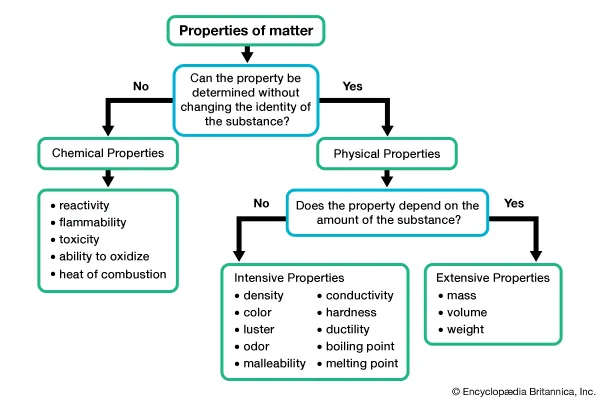
\includegraphics[width=0.9\textwidth]{matter_flowchart}
	\caption{Properties of Matter Flowchart. \note{Remember the difference between Intensive and Extensive physical properties}}
\end{figure}

\subsection{Changes in Matter}

Physical changes to matter change a substance's physical appearance but not its chemical composition, and chemical changes affect its chemical composition (and usually additionally change its physical qualities in the process) \textbf{to form a completely new substance}. Physical changes include melting ice, forming clouds, cutting, breaking, etc. Chemical changes include heating/cooking, reacting a substance with another substance, healing a wound, rusting, fermentation, etc. \\

\noindent
\note{Remember that the key difference between physical and chemical changes is whether or not a new substance is formed by the change.} \\

\noindent
\note{Dissolving salt into water is actually a chemical change because when salt dissolves, it dissociates into ions, thus changing its chemical composition, but dissolving sugar into water is physical because the sugar simply changes from a solid state to an aqueous state.}

\subsubsection{Naming Changes Between Matter States}

The movement from each state of matter to another has a completely different term based on the nature of the change.

\begin{figure}[H]
	\centering
	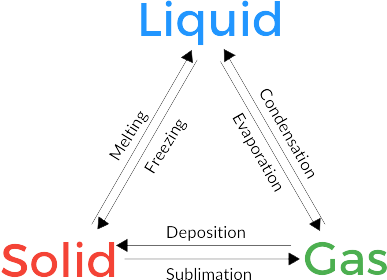
\includegraphics[width=0.6\textwidth]{state_triangle}
	\caption{States of Matter Flowchart}
\end{figure}

\newpage

\subsection{Pure Substances and Mixtures}

Matter can be classified into one of two types: mixtures or pure substances. Pure substances are composed of a singular substance and cannot be physically separated (think like Pure Gold). Whereas mixtures are comprised of more than one substance and can be physically separated into its component substances.

\begin{figure}[H]
	\centering
	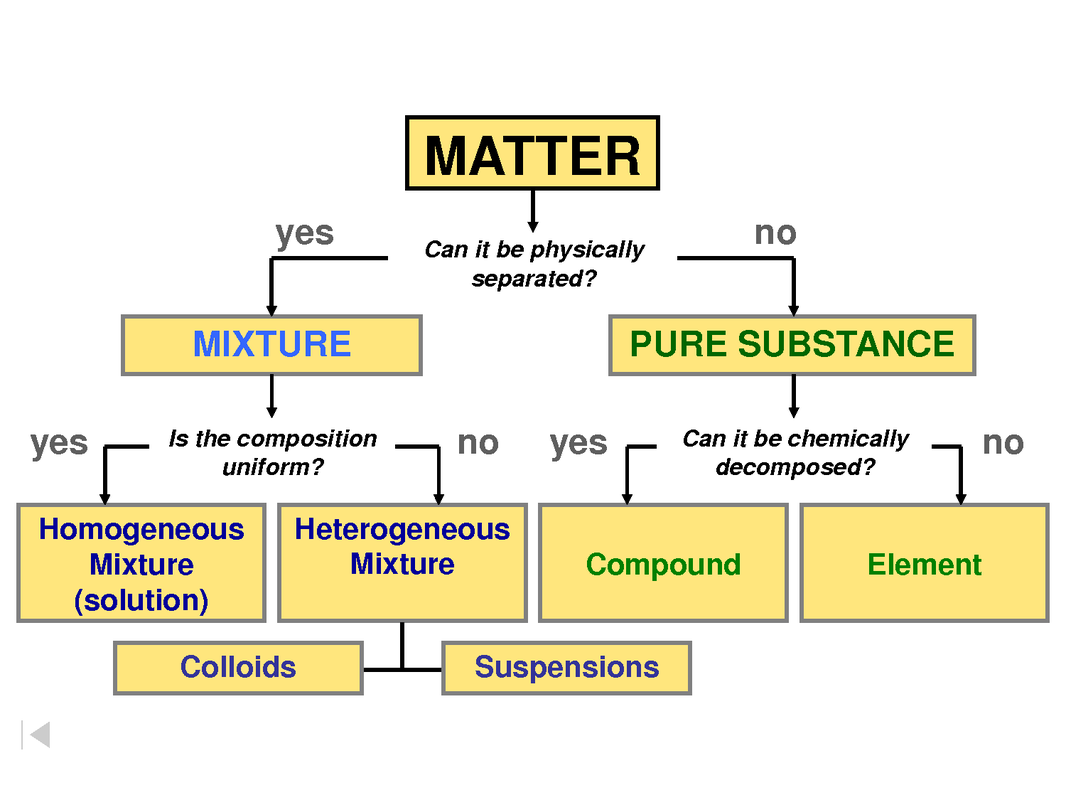
\includegraphics[width=\textwidth]{matter_types_flowchart}
	\caption{Pure Substance vs. Mixtures Flowchart}
\end{figure}

\begin{itemize}
\item \textit{Pure Substances} only ever have one substance present, and thus, have a definite and constant composition and consistent chemical and physical properties. \note{Pure substances are always chemically homogeneous, but they can be physically homogeneous or heterogeneous.}
\item \textit{Mixtures} are combinations of more than one type of substance, and thus, have variable composition and properties. \note{Mixtures are always chemically heterogeneous but, like pure substances, can be physically homogeneous or heterogeneous.}
\item \textit{Elements} are molecules with a singular \textit{type} of atom.
\item \textit{Compounds} are molecules with two or more types of atoms joined together.
\item \textit{Homogeneous Mixtures} are mixtures where a substance (known as the solute, such as salt or sugar) is dissolved into another substance (known as the solvent, such as water) at a \textit{uniform distribution} (think saltwater). These mixtures are also known as \textbf{solutions} and have one distinct physical appearance (or phase).
\item \textit{Heterogeneous Mixtures} are non-solution mixtures with a non-uniform distribution of its comprising particles and thus, two or more distinct physical appearances/phases (think Chex Mix).
\end{itemize}

\subsection{Elements and Compounds}

\begin{defn}
Elements are the building blocks of all higher types of matter and are made from atoms. They are the smallest classification of substances, and thus, cannot be broken down into simpler substances through chemical or physical means. \note{There are currently 118 known atom types, and 90 of those types occur naturally in nature.}
\end{defn}



\chapter{Elements}
\section{Lecture 1: Subatomic Particles and Isotopes}

Matter consists of various mixtures of substances comprised of molecules of compounds comprised of elements comprised of atoms, which are in turn comprised of protons, neutrons, and electrons.

\subsection{The Atomic Theory of Matter}

\begin{enumerate}
\item All matter is made of atoms, and each distinct type of atom is known as an element. (118 different types of which are currently known.)
\item All atoms of a given type will be similar to one another and different from all others.
\item Relative number and arrangement of different types of atoms in a pure substance determine its identity.
\item Chemical change is a \textit{union, separation, or rearrangement} of atoms to produce new substances.
\item Only whole atoms can participate in or result from any chemical change, and \textbf{for the purposes of this course, atoms are considered indestructible during chemical changes.}
\end{enumerate}

\subsection{Molecules}

\begin{defn}
Molecules are made from two or more atoms bonded \textbf{convalently} to function as a singular entity, known as a \textit{molecular compound}. In a molecule, \textit{the relative number and arrangement of its atoms} determine its identity.
\end{defn}

\noindent
\note{Whereas the atom is the limit of chemical subdivision, the molecule is the limit of physical subdivision.}

\begin{itemize}
\item There is only ever one type of molecule for any given molecular substance (otherwise it is a mixture).
\item Molecules have their own properties which will be different from their individual atoms.
\end{itemize}

\subsubsection{Molecule Types}

\begin{itemize}
\item Diatomic Molecule: Two atoms
\item Polyatomic Molecule: More than one atoms
\item Homoatomic Molecule: The atoms in the molecules are the same type
\item Heteroatomic Molecule: The atoms in the molecules are different types
\end{itemize}

\noindent
\note{There are seven elements that naturally exist as diatomic molecules: Hydrogen (H$_{2}$), Nitrogen (N$_{2}$), Oxygen (O$_{2}$), Flourine (F$_{2}$), Chlorine (Cl$_{2}$), Bromine (Br$_{2}$), and Iodine (I$_{2}$).}

\begin{itemize}
\item Molecules containing Carbon are called \textbf{organic}.
\item Molecules containing \textbf{only} Carbon, Hydrogen, and Oxygen are called \textbf{carbohydrates}.
\item Molecules that only contain Caybon and Hydrogen are called \textbf{Hydrocarbons}.
\end{itemize}

\subsection{Atoms}

\begin{itemize}
\item Atoms are always neutral, as they always have the same number of protons and electrons. This balance is broken in \textbf{ions}.
\item Atoms make up elements and compounds.
\item Individual atoms are smaller than the wavelength of light, so they cannot be seen with an optical microscope.
\item The mass of the atom lies solely in the nucleus, but the vast majority of the atom's size is in the electron cloud. (The ratio of the size of the electron cloud to the nucleus is 1 to 100,000.)
\end{itemize}

\begin{figure}[H]
	\centering
	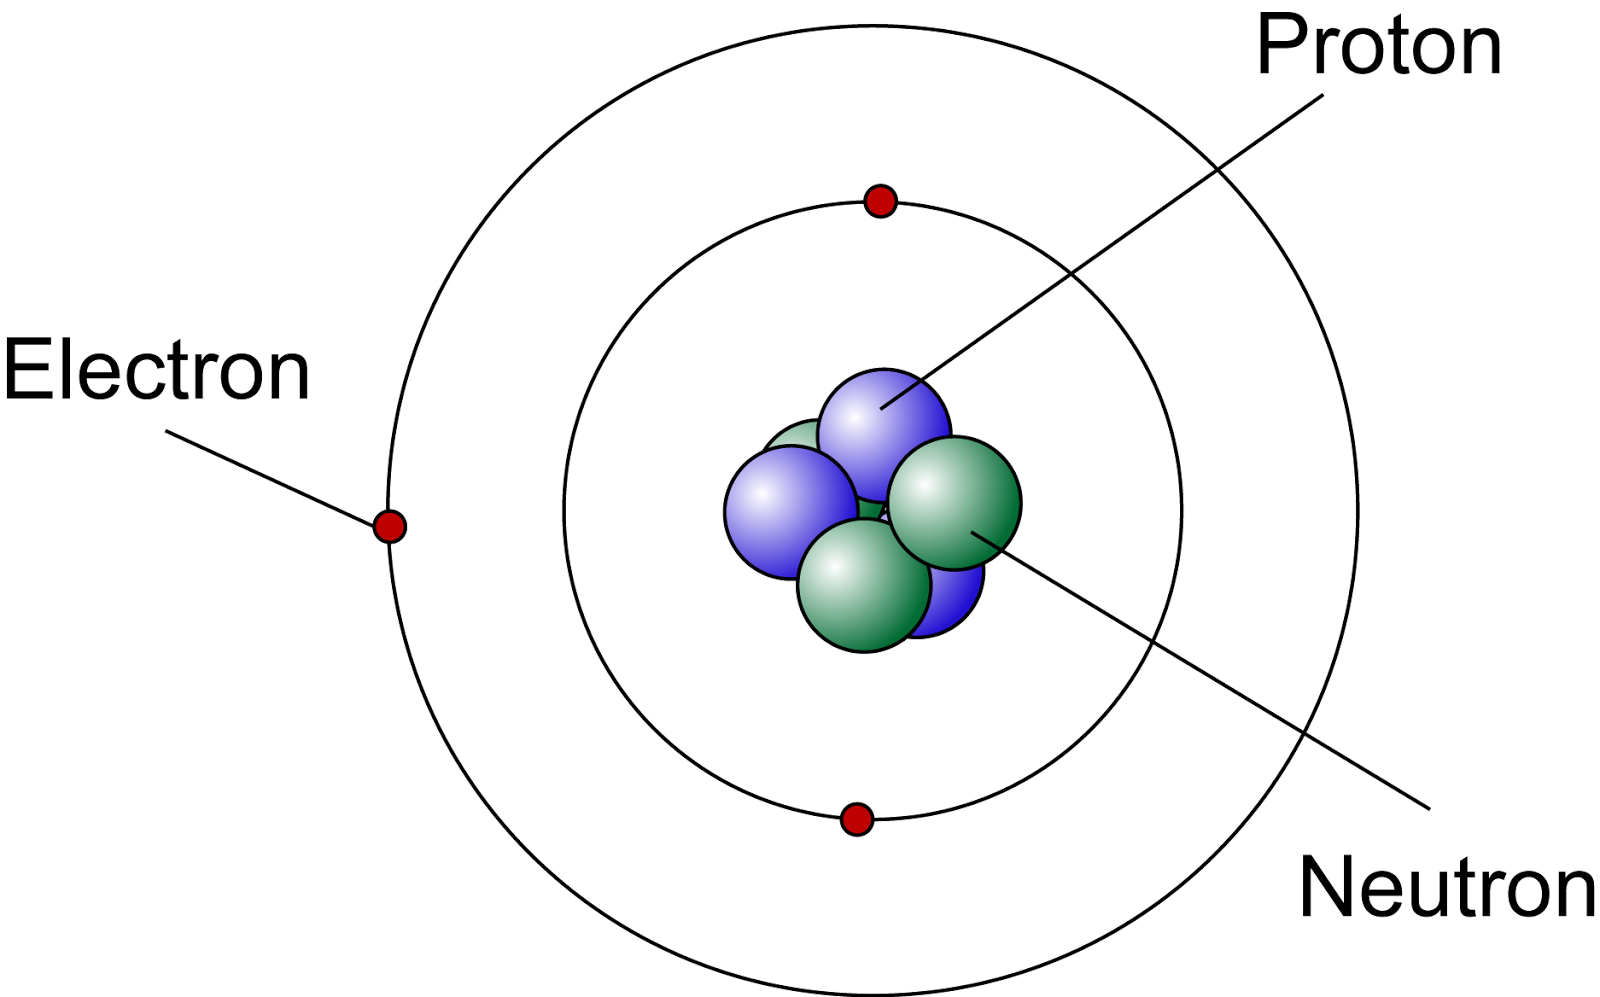
\includegraphics[width=\textwidth]{atom_model}
	\caption{Chadwick's Model of an Atom}
\end{figure}

\subsection{Subatomic Particles}

\begin{defn}
Atoms are comprised of smaller fundamental particles known as subatomic particles. The three core subatomic particles are \textbf{Protons, Neutrons, and Electrons}.

\begin{itemize}
\item Protons have a positive charge and weigh slightly less (but effectively equal to) a Neutron.
\item Neutrons have no/neutrual charge and weigh the most out of the previous two particles.
\item Electrons have a negative charge and weigh roughly 1800 times less than Protons and Neutrons, with effectively no mass.
\end{itemize}
\end{defn}

\noindent
The atom is split into two key portions, the nucleus and the electron cloud. The nucleus is the small, incredibly dense center of the atom that contains its protons and neutrons (which \textit{always results in a positive charge}), and these protons and neutrons within the nucleus are referred to as \textit{nucleons}. The electron cloud is the large outer region of the atom where the electrons move freely and rapidly throughout the nucleus, \textit{thus always resulting in a negative charge}. It has no firmly defined area for any atom and contains various shell and subshell levels which contain orbitals for the electrons.

\subsubsection{Nuclear Notation}

Nuclear Notation is used to indicate the atomic number and mass number of an atom of isotope, and it is formed by writing an elemental symbol preceded by a subscript indicating its atomic number (Z) and a superscript indicating its mass number (A). \\

\noindent
\note{Together, an atom with a specific atomic number and a specific mass number form a \textbf{nuclide.}}

\begin{figure}[H]
	\centering
	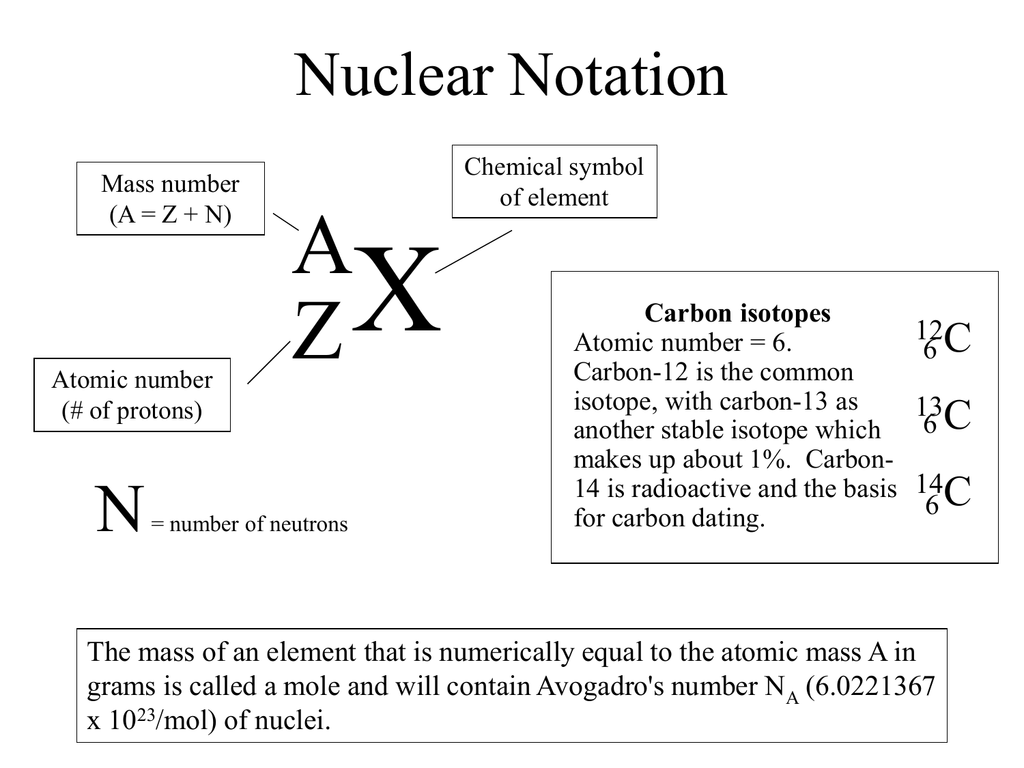
\includegraphics[width=\textwidth]{nuclear_notation}
	\caption{Nuclear Notation Model}
\end{figure}

\begin{defn}
The Atomic Number, denoted by Z, is the number of protons in the nucleus of the atom, and it acts as the primary definition of each type of atom (or Element). Atomic Numbers 1 through 92 (excluding Technetium and Promethium) are naturally occuring and the remaining 93 through 118 are synthetic. \note{As Atoms always hold a neutral charge, the number of electrons will always equal the number of protons and the atomic number.} \\

\noindent
The Mass Number is the sum of the number of protons and neutrons within the nucleus of an atom, and it is a count, \textbf{not} an atomic mass.
\end{defn}

\subsection{Isotopes}

\begin{defn}
Isotopes are atoms of an element that have the same number of protons and electrons but a different number of neutrons, and they are named by denoting the name of the element followed by its newfound mass number (such as Cobalt-60 or Carbon-14).
\end{defn}

\noindent
As an element is determined by the number of protons in the nucleus, the nucleus can have a variable number of neutrons without changing the charge but resulting in changes to the atom's mass number, and this change results in slightly different physical properties but generally similar chemical properties. \\

\noindent
\note{The mass number minus the atomic number is equal to the number of neutrons present in an isotope.}

\subsubsection{Isobars}

\begin{defn}
Isobars are atoms/nuclides of different chemical elements that have the same number of nucleons. Examples include Iron-58 (\ce{^{58}_{26}Fe}) and Nickel-58 (\ce{^{58}_{27}Ni}), or Calcium-40 (\ce{^{40}_{20}Ca}) and Argon-40 (\ce{^{40}_{18}Ar}).
\end{defn}

\subsection{Atomic Mass}

\begin{defn}
The atomic mass is a weighted average that accounts for the number of isotopes for the element, the percent abundance of each isotope, and the relative mass of each isotope (with Carbon-12 as the reference point).
\end{defn}

\section{Lecture 2: Electronic Structure and Chemical Periodicity}

\textbf{References chapter 4, sections 4.4 to 4.7 of the textbook.}

\subsection{The Periodic Table}

\begin{defn}
\textbf{The Periodic Law} \\

\noindent
When elements are arranged in order of increasing atomic number, elements with similar chemical behavior occur at regularly recurring (or \textit{periodic}) intervals.
\end{defn}

\begin{itemize}
\item Period: The horizontal row of elements in the periodic table.
\item Group: The verticle column of elements in the periodic table.
	\begin{itemize}
	\item There are three ways to name the columns: US, EU, and IUPAC
	\item There are four groups with non-numerical names: Alkali Metals, Alkali Earth Metals, Halogens, and Nobel Gases
	\end{itemize}
\item Chemical Periodicity: The variation in properties of elements as a function of their position on the periodic table (or how atoms change as they travel up/down the periodic table).
	\begin{itemize}
	\item There are three properties of elements that exhibit chemical periodicity: metallic vs. non-metallic character, atomic size, and electronegativity.
	\end{itemize}
\end{itemize}

\noindent
\note{Increasing atomic number \textbf{does not} always equal increasing atomic mass.} \\

\noindent
Elements in the periodic table can be classified in one of two ways: either by their electron configurations (nobel gases, representative elements, transition metals, or inner transition/rare earth metals) or their physical properties (metals/non-metals/metalloids)

\subsubsection{Representative Elements}

\begin{defn}
Representative elements are all of the elements located in the first two columns (denoted as the \elvl{s} area) or columns 13-17 (denoted as the \elvl{p} area).
\end{defn}

\noindent
Most elements are representative elements, and they generally have a partially or completely full \elvl{s} electron level and either an empty or partially filled \elvl{p} electron level.

\subsubsection{Alkali Metals (Group IA)}

\begin{itemize}
\item Members: Lithium (Li), Sodium (Na), Potassium (K), Rubidium (Rb), and Cesium (or Caesium) (Cs)
\item They only have one valence electron.
\item All soft, shiny metals.
\item All very reactive with water.
\end{itemize}

\subsubsection{Alkaline Earth Metals (Group IIA)}

\begin{itemize}
\item Members: Beryllium (Be), Magnesium (Mg), Calcium (Ca), Strontium (St), and Barium (Ba)
\item They all have two valence electrons.
\item All soft, shiny metals.
\item Only moderately reactive with water.
\end{itemize}

\subsubsection{Halogens (Group VIIA)}

\begin{itemize}
\item Members: Flourine (F), Chlorine (Cl), Bromine (Br), Iodine (I), and Astatine (At)
\item They all have seven valence electrons.
\item They all exist as diatomic molecules.
\item They are all very reactive colored substances.
\item Almost all are all gases at room temperature (or slightly above room temperature), except for Bromine, which is a liquid at room temperature.
\end{itemize}

\subsubsection{Noble Gases}


\begin{itemize}
\item Members: Helium, Neon, Argon, Krypton, Xenon, and Radon
\item They all have a full valence shell of electrons.
\item They are all completely unreactive (hence the name "Noble," as they are too noble to react with other substances).
\item They are all gases at room temperature.
\end{itemize}

\subsubsection{Transition Element}

\begin{defn}
Transition elements are located in the \elvl{d} area of the periodic table, and their electrons fill the \elvl{D} energy level.
\end{defn}

\subsubsection{Inner Transition Element}

\begin{defn}
Inner Transition Elements are located in the \elvl{f} area of the periodic table, and their electrons fill the \elvl{f} energy level. This series are referred to as \textbf{Lanthanides and Actinides} and are generally known as "Rare Earth Elements."
\end{defn}

\subsection{Physical Properties of Table Elements}

\subsubsection{Metals}

\begin{itemize}
\item Luster (Shine)
\item Thermal Conductivity
\item Electrical Conductivity
\item Malleability (can be rolled into sheets)
\item Ductility (can be drawn into wires)
\item All solids at room temperature (except for Mercury)
\item High Density
\item High Melting Point
\end{itemize}

\noindent
\note{There are 94 actively known metals.}

\subsubsection{Non-Metals}

\noindent
\note{Non-metals are generally characterized by their lack of the properties of \textit{luster, thermal conductivity, electrical conductivity, and malleability} in reference to metals.}

\begin{itemize}
\item Can be solids, liquids, or gases at room temperature.
	\begin{itemize}
	\item Nitrogen (N), Oxygen (O), Hydrogen (H), Chlorine (Cl), Flourine (F), Helium (He), Neon (Ne), Argon (Ar), Krypton (Kr), Xenon (Xe), and Radon (Rn) are all \textbf{gases}.
	\item Carbon (C), Phosphorus (P), Sulfur (S), Selenium (Se), Iodine (I), Astatine (At), and Tellurium (Te) are all \textbf{solids}.
	\item Bromine (Br) is a \textbf{liquid}.
	\end{itemize}
\item Generally have lower density and lower melting points than metals.
\end{itemize}

\subsection{Periodic Table Trends}

\subsubsection{Metallic Character}

\begin{defn}
Metallic character is a general chemical property that describing how `metallic' an element is, and for any given period/row in the periodic table, it increases from right to left, and for any given group, it increases going top to bottom. For example, Sodium (Na) is more Metallic than Magnesium (Mg) but less metallic than Potassium (K).
\end{defn}

\subsubsection{Non-Metallic Character}

\begin{defn}
Non-metallic character is another general chemical property that describes how `non-metallic' an element is (and subsequently, it works in the exact opposite manner to metallic character). As such, for any given period, it increases from left to right, and for any given group, it increases going bottom to top. For example, Chlorine (Cl) is more non-metallic than Phosphorus (P) but less non-metallic than Flourine (F).
\end{defn}

\subsubsection{Metalloids and Semiconductors}

\begin{defn}
Metalloids are an element whose properties intermediate between those of metals and non-metals, and there are eight known metalloids: Boron (B), Sillicon (Si), Germanium (Ge), Arsenic (As), Antimony (Sb), Tellurium (Te), Polonium (Po), and Astatine (At).
\end{defn}

\noindent
\note{Metalloids reside along the stepped line which divides the metals and non-metals.}

\begin{defn}
Semiconductors are metalloids that do not conduct electrical currents at room temperatures but are able to conduct electrical currents at higher temperatures, and there are three main semiconductors: Sillicon (Si), Germanium (Ge), and Antimony (Sb).
\end{defn}

\noindent
\note{Semiconductors are vital in the electronics industry.}

\subsubsection{Atomic Size}

Atomic Radii tend to increase from right to left within any given period and increase from top to bottom for any given group. For example, Helium is rougly the smallest whereas Francium is roughly the largest.

\subsubsection{Electronegativity}

\begin{defn}
Electronegativity is a measure of the relative attraction that an atom has for the shared electrons within its bonds.
\end{defn}

\begin{itemize}
\item The higher the electronegativity of an element, the greater the electon-attracting ability of the atoms of that element.
\item Electronegativity generally increases from left to right within a given period and from bottom to top within a given group.
\item Electronegativity depends on numerous factors: atomic size, nuclear charge, and the number of non-valence electrons.
\end{itemize}

\subsection{Electon Shells, Subshells, and Orbitals}

\subsubsection{Base Review of Electrons}

\begin{itemize}
\item Electrons are the smallest of the three main subatomic particles.
\item Electrons have very small mass.
\item They reside in the electron cloud surrounding the nucleus.
\item Their rapid movement around the nucleus defines the size of the atom.
\item The information regarding the behavior and the arrangements of electrons outside of the nucleus is definved from quantum mechanics.
\item Electrons have spin.
\item Energy in an electron is defined and restricted, so it cannot just go `anywhere.'
\item An energy on electrons is quantized, meaning that it can only have certain values.
\end{itemize}

\subsubsection{Electron Shells}

\begin{defn}
An \textbf{electron shell} is a defined region of space about a nucleus that only contains electrons with approximately the same energy. The \textbf{shell number}, \elvl{n}, is used to identify the electron shell. Electron shells are numbered 1 to 7, and electrons in higher shell numbers have more energy.
\end{defn}

\begin{itemize}
\item Not all electron shells have an equal number of electrons.
\item The number of electrons in a shell generally follows the formula $N = 2n^{2}$, where \elvl{n} is the electron shell level. (I.e., level 3 would have $2(3)^{2}$ or 18 electrons.) 
\item Lower level shells fill before higher ones.
\end{itemize}

\subsubsection{Electron Subshells}

Within an electron shell, there are subshells and orbitals. A subshell is a defined region of space within an electron shell that contains electrons of the same energy level, such as \elvl{s}, \elvl{p}, \elvl{d}, or \elvl{f}.

\begin{itemize}
\item The number of subshells in an electron shell is equal to the shell number.
\item The number of electons in each subshell is defined and independent of the shell number.
\begin{multicols}{2}
	\begin{itemize}
	\item \elvl{s} has 2 electrons.
	\item \elvl{p} has 6 electrons.
	\item \elvl{d} has 10 electrons.
	\item \elvl{f} has 14 electrons.
	\end{itemize}
\end{multicols}
\item Electron subshells are denoted by the electron shell number followed by the letter of the electron subshell with a superscript denoting the number of the number of electrons in the given subshell, such as $1s^{2}$.
\end{itemize}

\subsubsection{Electron Orbitals}

\begin{defn}
Electron orbitals are regions of space within an electron subshell where with a specific energy is most likely to be found.
\end{defn}

\noindent
\note{The number of orbitals in each subshell is one-half of the number of electrons within the subshell, as each orbital can hold two electrons.}

\begin{multicols}{2}
\begin{itemize}
\item \elvl{s} has 1 orbital.
\item \elvl{p} has 3 orbitals.
\item \elvl{d} has 10 orbitals.
\item \elvl{f} has 14 orbitals.
\end{itemize}
\end{multicols}

\subsubsection{The Aufbau Principle}

Electron shells fill according to the \textit{Aufbau Principle}, wherein electrons normally occupy electron subshells in an atom in order of increasing subshell energy, and the energy of subshells can overlap.

\subsection{Electron Configuration}

\begin{defn}
Electron configuration serves as a shorthand notation describing the sbushells in an atom that are occupied by electrons.
\end{defn}

\noindent
Electron configuration is written by starting at the beginning (no electrons) and then continuously filling electron subshells until the correct number of electrons are represented. (Example table below)

\begin{table}[H]
\centering
\begin{tabular}{|c|c|l|}
\hline
Element & Number of Protons (Z) & Electron Configuration \\
\hline
Hydrogen & 1 & $1s^{1}$ \\
\hline
Helium & 2 & $1s^{2}$ \\
\hline
Carbon & 6 & $1s^{2} 2s^{2} 2p^{2}$ \\
\hline
Neon & 10 & $1s^{2} 2s^{2} 2p^{6}$ \\
\hline
Sodium & 11 & $1s^{2} 2s^{2} 2p^{6} 3s^{1}$ \\
\hline
Potassium & 19 & $1s^{2} 2s^{2} 2p^{6} 3s^{2} 3p^{6} 4s^{1}$ \\
\hline
Rubidium & 37 & $1s^{2} 2s^{2} 2p^{6} 3s^{2} 3p^{6} 4s^{2} 3d^{10} 4p^{6} 5s^{1}$ \\
\hline
Cesium & 55 & $1s^{2} 2s^{2} 2p^{6} 3s^{2} 3p^{6} 4s^{2} 3d^{10} 4p^{6} 5s^{2} 4d^{10} 5p^{6} 6s^{1}$ \\
\hline
\end{tabular}
\end{table}

\begin{figure}[H]
	\centering
	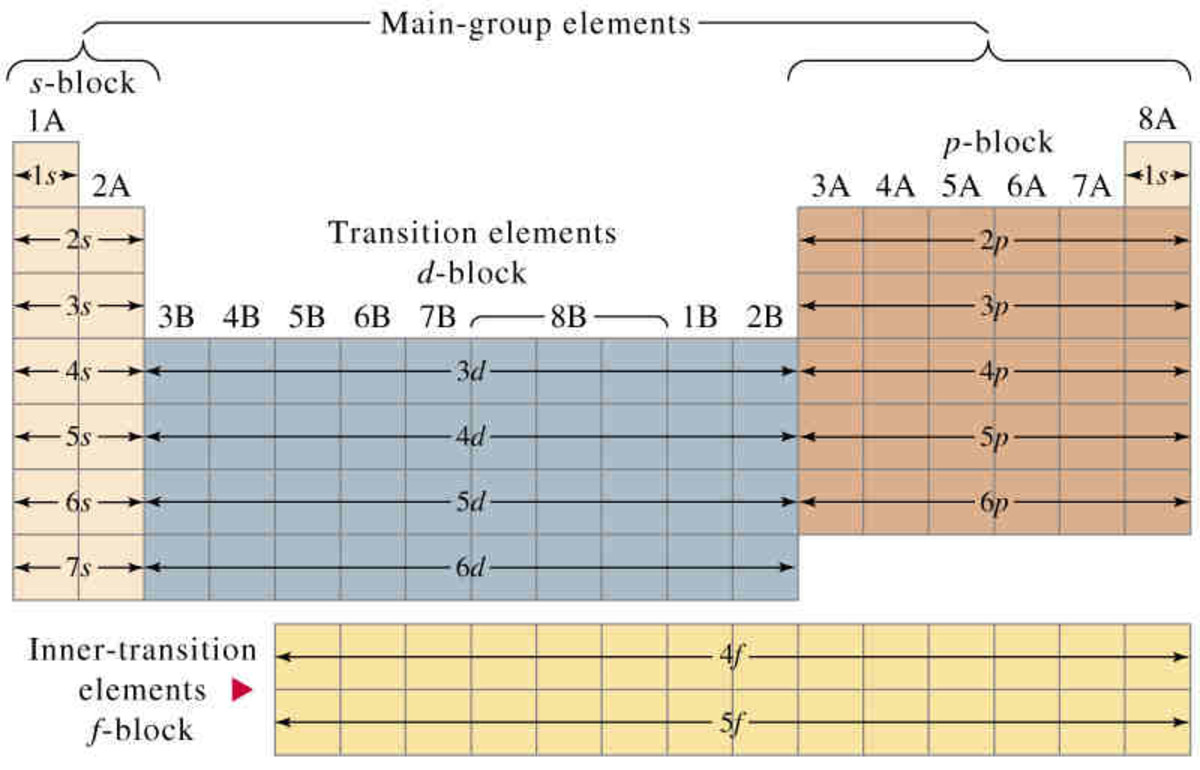
\includegraphics[width=\textwidth]{electron_configuration_table}
	\caption{Ground State Electron Configurations of the Elements}
\end{figure}

\subsubsection{Condensed Electron Configuration}

Electron configuration can also be condensed by utilizing a starting point element (commonly a noble gas) surrounded by brackets then continuing the electron configuration from there. \\

\noindent
For example, as Sodium's electron configuration is $1s^{2} 2s^{2} 2p^{6} 3s^{1}$ and Neon's electron configuration is $1s^{2} 2s^{2} 2p^{6}$, one could condense the electron configuration for Sodium down to [Ne]$3s^{1}$. \\

\noindent
\note{For \elvl{d}, use one less than the period, and for \elvl{f}, use two less than the period.}

\subsection{Paramagnetic and Diamagnetic Substances}

\begin{itemize}
\item Atoms where all electron orbitals are occupied by pairs of electrons are called \textit{diamagnetic} atoms.
\item Atoms where all electron orbits are not occupied by pairs of electrons are called \textit{paramagnetic} atoms.
\end{itemize}

\subsubsection{Visualizing Electron Orbitals}

We can visualize electron orbitals using arrows. Levels that are completely filled are diamagnetic and those that are not are paramagnetic.

\begin{figure}[H]
	\centering
	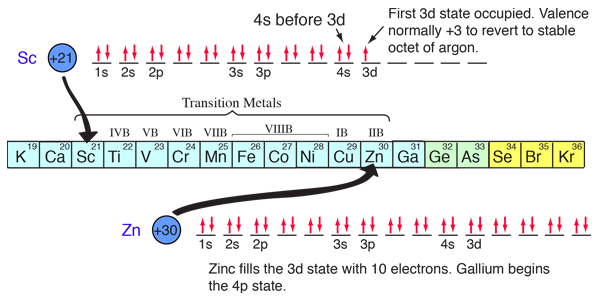
\includegraphics[width=\textwidth]{electron_orbitals_visualization}
	\caption{Electron orbitals visualized with arrows. In this diagram, Scandium (Sc) is paramagnetic and Zinc (Zn) is diamagnetic.}
\end{figure}


\chapter{Compounds}
\section{Lecture 1: Ionic and Covalent Compounds}
\textbf{References chapter 5 of the textbook.}

\subsection{Types of Chemical Bonds}

There are two main types of chemical compounds: ionic compounds and molecular compounds. \\

\noindent
\note{The attractive forces that hold atoms together are called chemical bonds.}

\begin{defn}
An ionic bond is a chemical bond formed through the tranfer of electrons from one atom (or group of atoms) to another to form ions. A covalent bond is a chemical bond formed through the sharing of electron \textbf{pairs} between atoms.
\end{defn}

\begin{table}[H]
\noindent\makebox[\textwidth]{
\begin{tabular}{|l|p{0.4\textwidth}|p{0.4\textwidth}|}
\hline
\textbf{Property} & \textbf{Ionic Bond} & \textbf{Covalent Bond} \\
\hline
Chemical Formula & Formula Unit & Molecular Formula \\
\hline
Molecule Discreteness & No Discrete Molecule & Forms Discrete Molecules \\
\hline
Melting Point & High Melting Point & Lower Melting Points \\
\hline
Electrical Conductivity & Good Conductors when Molten & Cannot Conduct \\
\hline
Solubility & Soluble in Polar Solvents and Not Soluble in Non-Polar Solvents & Soluble in Non-Polar Solvents and Some Polar Solvents \\
\hline
State of Matter & N/A & Gases, Liquids, and Low-Melting Solids \\
\hline
\end{tabular}}
\end{table}

\noindent
\note{Chemical bonds can be strongly ionic or strongly covalent, but they will usually be a mix of both.} \\

\noindent
\note{Only valence electrons are able to be utilized for bonding.} \\

\subsubsection{The Octet Rule}

Electron bonds occur to further stabilize a chemical or group of chemicals by reaching a state of completely full valence electrons. Thus, Noble Gases are entirely unreactive, as they already have completely full valence electrons. Through these bonds, electrons can either \textbf{lose, gain, or share} electrons to reach a full valence state (which would be the same configuration as any one of the noble gases). This process is often referred to as \textbf{the octet rule.}

\subsubsection{Lewis Dot Symbols}

\begin{defn}
A Lewis Dot Symbol is a chemical symbol of an element surrounded by dots equal to the number of valence electrons.
\end{defn}

\noindent
\note{The choice of where the dots are placed is not important.}

\subsection{Ionic Bonds}

\begin{defn}
Ions are atoms (or groups of atoms) that are electrically charged as the result of losing or gaining valence electrons. Anions are negatively charged (usually nonmetals), and cations are positively charged (usually metals).
\end{defn}

\noindent
Whether or not an element loses or gains electrons is dependent on how many valence electrons the element has. If the number of valence electrons is closer to 0, it is more likely to lose electrons, and if the number of valence electrons is closer to 8, it is more likely to gain electrons.  \\

\noindent
This property is why metals, which are generally closer to the left of the periodic table and thus have less valence electrons, are more likely to lose electrons, and non-metals, which are further to the right and thus have more valence electrons, and more likely to gain electrons. \\

\noindent
\note{By this rule, common ionic behavior is best observed in the representative elements (but not in the transition elements, as they have a more balanced number of valence electrons). Group 1 will normally have a 1+ charge, group 2 will normally have a 2+ charge, group 13 will have a 3+ charge, group 14 will have a 4+ or 4- charge, group 15 will have a 3- charge, group 16 will have a 2- charge, and group 17 will have a 1- charge.} \\

\noindent
Ions with the same electron configuration as a noble gas are considered \textbf{Isoelectronic} with athe noble gas, and \textbf{isoelectronic species} are the set of ions (and possibly an element as well) that all have the same electron configuration.

\subsubsection{Ionic Compound Formulas}

The net charge of every compound must be equal to zero, with positive ions written first and negative ions written after. Charges on each individual ions are not reflected in the formula, and subscript numbers in the formula give the combining ratio of the ions rather than the exact count. \\

\noindent
For example, in the ion \ce{NaCl}, Na carries a +1 charge and Cl carries a -1 charge. Thus, NaCl is neutral. 

\subsubsection{Ionic Compounds}

Ionic compounds are usually comprised of a metal and a nonmetal (also known as a \textbf{polyatomic} ion), and the ratio in which these ions combine is always the lowest possible ratio that garners a net neutral charge between the two. These ratios are known as \textbf{Formula Units}. \\

\noindent
\note{Metals are groups IA (1), IIA (2), and IIIA (13), and Non-Metals are groups VA (15), VIA (16), and VIIA (17).} \\

\noindent
Metallic atoms usually lose electrons and become positively charged, and non-metallic atoms usually gain electrons and become negatively charged.

\subsection{Covalent Bonds}

\begin{defn}
Covalent bonds are bonds between two non-metal atoms as a result of two atoms \textbf{sharing} the same valence electrons.
\end{defn}

\begin{figure}[H]
	\centering
	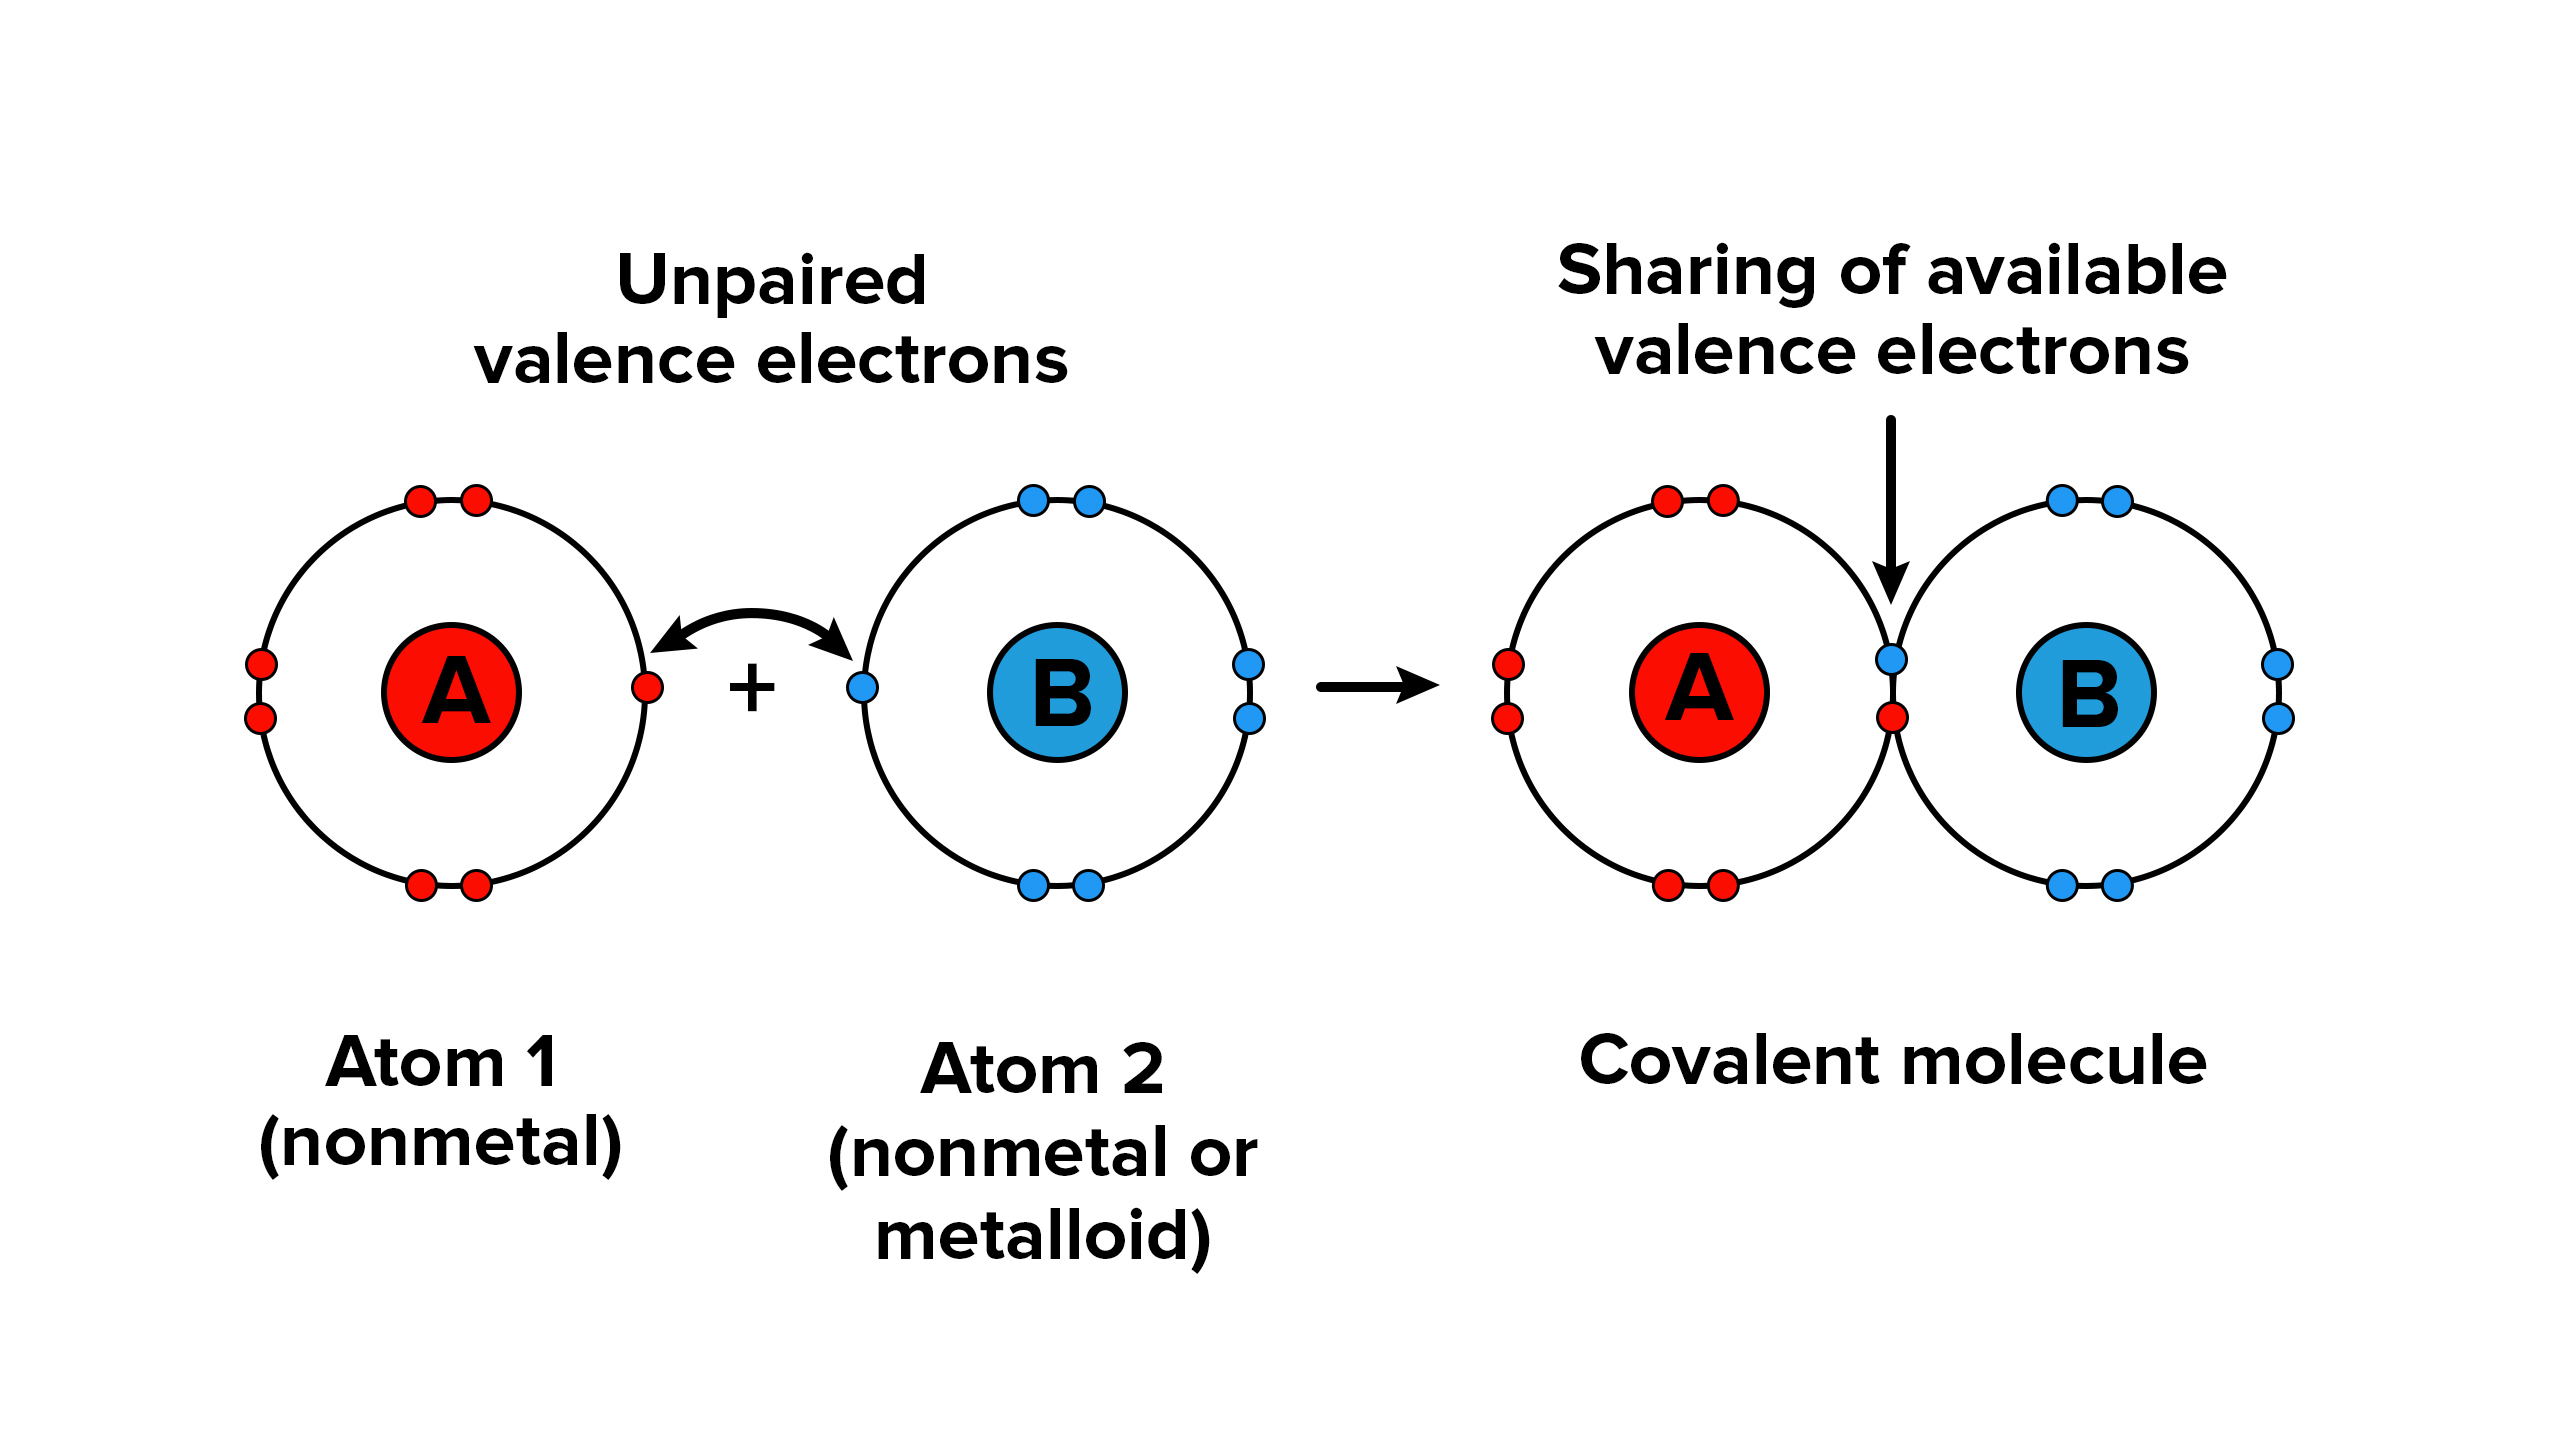
\includegraphics[width=\textwidth]{covalent_bond}
	\caption{Covalent Bond}
\end{figure}

\noindent
Atoms in covalent bonds can have both bonding electrons and non-bonding electrons, where the shared electrons are considered `bonding.' \\

\noindent
\note{Covalent compounds can form single, double, or triple bonds by sharing one, two, or three pairs of electrons, with each bond represented with a straight line.}

\subsection{Molecular Geometry and VSEPR}

\begin{defn}
Molecular Geometry is a description of the three dimensional arrangement of atoms within a molecule, and it plays a critical role in determining the physical and chemical properties of substances.
\end{defn}

\begin{defn}
Valence Shell Electron Pair Repulsion Theory, or VSEPR Theory, is a set of procedures for predicting the geometric structure of a molecule from its lewis dot structure.
\end{defn}

\noindent
In VSEPR, the non-binding electron pairs and the number of atoms bonded to an atom determine the geometric structure of an atom as \textbf{electrons naturally repel each other}. (\note{this is why remembering the number of electron groups is key.}) \\

\noindent
A VSEPR electron group is a group of valence electrons around an atom or molecule. (\note{It is slightly different from an electron pair.})

\subsubsection{The Core of Molecular Geometry based on VSEPR}

\begin{enumerate}
\item Atoms arrange themselves to be as far from other electrons as possible.
\item There is no distinction made between bonding/shared electrons and non-bonding/lone electrons.
\item Single, double, and triple bonds are all counted equally as one pair attached to the central atom.
\end{enumerate}

\subsubsection{Types of VSEPR Configurations}

\begin{figure}[H]
	\centering
	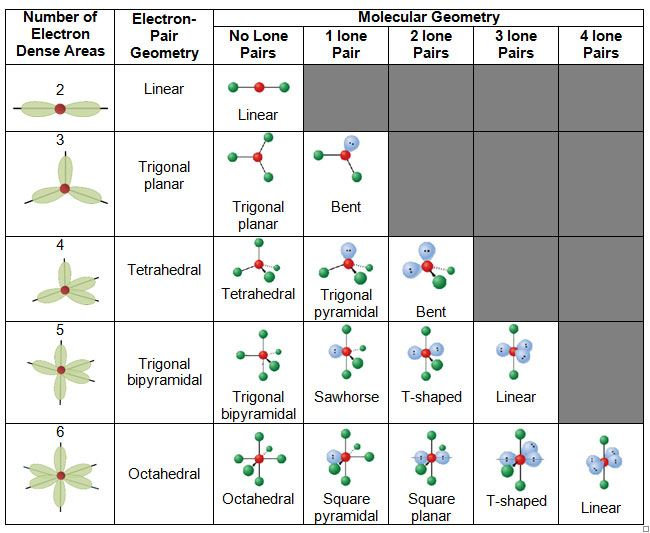
\includegraphics[width=\textwidth]{vsepr_table.jpg}
	\caption{Types of VSEPR Configurations}
\end{figure}

\begin{itemize}
\item Molecules with 2 or 3 VSEPR pairs are \textbf{planar}.
\item Molecules with VSEPR pairs that are strictly $180^\circ$ apart are \textbf{linear}.
\item Molecules with VSEPR pairs that are strictly $120^\circ$ will be \textbf{Triagonal Planar} or \textbf{Angular/Bent}.
\item Molecules with VSEPR pairs that are strictly $109.5^\circ$ will be either \textbf{Tetrahedral,  Trigonal Pyramidal, or Angular/Bent}
\end{itemize}

\begin{table}[H]
\centering
\begin{tabular}{|l|l|l|}
\hline
\textbf{Formula} & \textbf{VSEPR Groups} & \textbf{Shape} \\
\hline
\ce{XB2}   & 2 & Linear \\
\ce{XB3}   & 3 & Trigonal Planar \\
\ce{XB2N1} & 3 & Bent \\
\ce{XB4}   & 4 & Tetrahedral \\
\ce{XB3N1} & 4 & Trigonal Pyramidal \\
\ce{XB2N2} & 4 & Bent \\ 
\hline
\end{tabular}
\caption{X is the Central Atom, B is the Bonding Electron Groups, and N is the Non-Bonding Electron Groups.}
\end{table}

\subsection{Bond Polarity}

The greater the electronegativity of an atom, the greater its electron attraction. By this rule, atoms with different electronegativities will have bonds of different strengths.

\begin{defn}
\textbf{Bond Polarity} is the measure of the magnitude of difference in electron bonds between atoms.
\end{defn}

\begin{itemize}
\item Bonds with equal sharing of electrons are called non-polar covalent bonds.
\item Bonds that do not have an equal sharing of electons are known as polar covalent bonds and are represented with a "D-" or "D+" for negative and positive respectively.
\item Polar covalent bonds create a polarity in the resulting molecule, which influences its resulting properties.
\end{itemize}

\subsubsection{Calculating Bond Polarity}

Electronegativity differences can be used as a rough measure of calculating bond polarity given the following rules:


\begin{table}[H]
\centering
\begin{tabular}{|l|l|}
\hline
\textbf{Electronegativity Range} & \textbf{Bond Polarity Type} \\
\hline
$\Delta \chi < 0.4$ 		& Non-Polar Covalent \\
$0.4 \le \Delta \chi < 2$  	& Polar Covalent \\
$2 \ge \Delta \chi$			& Ionic \\
\hline
\end{tabular}
\caption{$\Delta \chi$ is the magnitude of difference between the electronegativities between the two elements.}
\end{table}

\noindent
For example, Hydrogen has an electronegativity of 2.1 and Chlorine has an electronegativity of 3.0, causing a difference of $\Delta \chi = 0.9$, and thus, a polar covalent bond. \textit{The greater this difference, the higher the polarity.} \\

\noindent
\note{Although the bonds can be polarized, sometimes the polarity can cancel out, causing the molecule to be non-polar.}

\subsection{Molecular Polarity}

\begin{defn}
Molecular Polarity is a measure of degree inequality in the attractiong of bonding electrons to various locations within a molecule, where polar molecules have unsymmetrical charge distribution and non-polar molecules have symmetrical charge distribution.
\end{defn}

\noindent
\note{Molecular geometry and bond polarity combined determine molecular polarity.}

\section{Lecture 2: Naming of Compounds}

The International Union of Pure and Applied Chemistry, or IUPAC, sets the following standard rules for naming compounds in chemistry.

\begin{itemize}
\item \textbf{Binary Ionic Compounds} contain a metal and a non-metal.
\item \textbf{Binary Molecular Compounds} consist of only non-metals. (\note{For naming purposes, metalloids are treated as non-metals.})
\item \textbf{Binary Acids} are compounds that release hydrogen ions when dissolved in water.
\end{itemize}

\subsection{Ionic Compounds}

\begin{itemize}
\item Ionic Compounds are the attraction between oppositely-charged ions, not atoms.
\item Ionic compounds form crystal lattices, not molecules.
\item The charge on an ionic compounds is always neutral.
\item Ionic compounds may contain one or more \textit{polyatomic ions.}
\end{itemize}

\subsubsection{Metal Ions}

\noindent
For naming purposes, there are two types of metal ions: fixed and variable charge.

\begin{defn}
\textbf{Fixed charge} ions are metal ions that form one type of positive ion that always have the same charge. \textbf{Variable charge} ions are metal ions that can form more than one type of positive ion.
\end{defn}

\noindent
The only fixed-charge ions are the metal elements in the IA, IIA, IB, IIB, and IIIA groups, or Lithium, Sodium, Potassium, Rubidium, Cesium, Beryllium, Magnesium, Calcium, Strontium, Barium, Aluminum, Gallium, Silver, Zinc, and Cadmium. \textit{All other metals have variable charge}, such as Chromium, Cobalt, or Gold.

\subsection{Naming Binary Ionic Compounds}

\begin{itemize}
\item When naming ionic compounds, positively-charged ions (cations) are named first, and negatively-charged ions (anions) are named after.
\item Metal ions (fixed or variable) take the name of the metal they come from.
\item Non-metal ions are named by taking the stem of the non-metal and adding the suffix "-ide."
\end{itemize}

\begin{example}
\ce{Li+} is a Lithium Ion, \ce{Mg^{2+}} is a Magnesium Ion, but \ce{Fl-} is a Fluoride ion and \ce{O^{2-}} is an Oxide ion.
\end{example}

\noindent
\note{Polyatomic ions always bring their own name to the compound.}

\begin{table}
\centering
\begin{tabular}{|l|l|l|l|}
\hline
\textbf{Element} & \textbf{Stem} & \textbf{Name of Ion} & \textbf{Formula} \\
\hline
Bromine   	& brom-	  & bromide   ion & \ce{Br-} \\
Carbon    	& carb-   & carbide   ion & \ce{C^{4-}} \\
Chlorine  	& chlor-  & chloride  ion & \ce{Cl-} \\
Fluorine	& fluor-  & fluoride  ion & \ce{F-} \\
Hydrogen	& hydr-   & hydride   ion & \ce{H-} \\
Iodine		& iod-    & iodide    ion & \ce{I-} \\
Nitrogen	& nitr-   & nitride   ion & \ce{N^{3-}} \\
Oxygen		& ox-	  & oxide 	  ion & \ce{O^{2-}} \\
Phosphorus 	& phosph- & phosphide ion & \ce{P^{3-}} \\
Sulfur		& sulf-   & sulfide   ion & \ce{S^{2-}} \\
\hline
\end{tabular}
\caption{Names for Common Non-Metal Ions}
\end{table}

\begin{example}
\ce{CaF2} would be Calcium flouride, and no importance is placed on the amount fo each element. 
\end{example}

\noindent
When naming binary ionic compounds with variable-charge metals, there has to be a differentiation between the different charges of the metal for situations such as differentiating between \ce{FeS} and \ce{Fe2S3} given the ions \ce{Fe^{2+}} and \ce{Fe^{3+}}.

\noindent
The solution to this is referring to each ion of the metal by its cation charge in roman numerals within parentheses, so \ce{Fe^{2+}} becomes Iron (II) and \ce{Fe^{3+}} becomes Iron (III).

\noindent
\note{If there is a metal in the compound, the metal is ionic.}

\subsection{Naming Compounds with Polyatomic Ions}

\begin{enumerate}
\item Most polyatomic ions are negatively charged, and the only two main positive ones are ammonium and hydonium.
\item Four polyatomic ions have names that end in "-ide" already: hydroxide, cyanide, azide, and peroxide.
\item Pay attention to the "-ate" and "-ite" pairs, as htey differ by the number of oxygen atoms, where "-ate" always has a greater number of oxygen atoms. For example, Sulfate (\ce{SO4^2-}) and Sulfite (\ce{SO3^2-}).
\item Some pairs differ by the addition of a hydrogen ion, such as Carbonate (\ce{CO3^2-}) and Hydrogen Carbonate (\ce{HCO3^2-}).
\item When Sulfur replaces an Oxygen atom, the prefix "Thio-" is added to the name, such as with Cyanate (\ce{OCN}) and Thiocyanate (\ce{SCN}) or Sulfate (\ce{SO4^2-}) and Thiosulfate (\ce{S2O3^2-}).
\end{enumerate}

\subsection{Binary Molecular Compounds}

Binary molecular compounds consist of two non-metal elements, and these compounds are named as the formula is written.

\begin{itemize}
\item The least electonegative element is named first.
\item The stem of the second non-metal follows with the suffix "-ide."
\item Numerical prefixes are used to indicate the number of both atoms present.
\end{itemize}

\noindent
\note{The number of atoms present is not clarified for polyatomic ions, but it is for binary molecular compounds.}

\begin{table}[H]
\centering
\begin{tabular}{|c|c|}
\hline
\textbf{Prefix} & \textbf{Value} \\
\hline
mono & 1 \\
di & 2 \\
tri & 3 \\
tetra & 4 \\
penta & 5 \\
hexa & 6 \\
hepta & 7 \\
octa & 8 \\
nona & 9 \\
deca & 10 \\
\hline
\end{tabular}
\end{table}

\noindent
\note{The exception to this rule is that binary compounds with hydrogen listed as the first element are named without using the prefix for how many atoms there are, and the prefix "mono" is always dropped at the beginning of a name.}

\subsubsection{Common Names to Know}

\begin{table}
\centering
\begin{tabular}{|l|l|}
\hline
\textbf{Formula Unit} & \textbf{Name} \\ 
\hline
\ce{H2O}  & Water \\
\ce{H2O2} & Hydrogen Peroxide \\
\ce{NH3}  & Ammonia \\
\ce{N2H4} & Hydrazine \\
\ce{CH4}  & Methane \\
\ce{C2H6} & Ethane \\
\ce{PH3}  & Phosphine \\
\ce{AsH3} & Arsine \\
\hline
\end{tabular}
\end{table}

\noindent
\note{The above examples are all binary compounds, but other molecular compounds with more than 2 elements don't follow these rules.} \\

\subsection{Introduction to Acids}

\begin{defn}
An acid is a hydrogen-containing molecular compound whose molecules yield Hydrogen ions (\ce{H+}) when dissolved in water (\ce{H2O}).
\end{defn}

\noindent
These acids can be identified by having Hydrogen as the first element shown in its formula, such as \ce{HCl}, \ce{H2S}, \ce{H2SO4}, or \ce{HNO3} (which are all acids), whereas \ce{NH3}, \ce{CH4}, \ce{PH3}, or \ce{SiH4} are all non-acidic. \\

\noindent
\note{Acids produce \ce{H+} in water, but an anion is also produced, depending on the structure of the molecular compound. For example, \ce{HCl} produces \ce{H+} and \ce{Cl-}.}

\subsubsection{Acid Nomenclature}

\begin{table}[H]
\centering
\begin{tabular}{|c|l|}
\hline
\textbf{Anion Ending} & \textbf{Acid Name} \\
\hline
"-ide" & hydro-\textit{(stem)}-ic acid \\
"-ate" & \textit{(stem)}-ic acid \\
"-ite" & \textit{(stem)}-ous acid \\
\hline
\end{tabular}
\end{table}

\subsection{Common Student Mistakes}

\begin{itemize}
\item For \textbf{ionic compounds ONLY}, formulas \textbf{must be reduced to its simplest ratios}. For example, \ce{Mn2O4} must be reduced to \ce{MnO2}.
\item Do not confuse Ammonia (\ce{NH3}) and an Ammonium Ion (\ce{NH4+}).
\item Chemical formulas do not show ionic charges. For example, write table salt as  \ce{NaCl}, not \ce{Na^{+}Cl^{-}}.
\item Don't put parentheses unless they are needed to show more than one of the same ion. For example, write \ce{NaNO3}, not \ce{Na(NO3)}
\end{itemize}




\chapter{Reactions}
\section{Lecture 1: Reactions}

\subsection{Introduction to Reactions}

\textbf{References Chapter 7, Sections 7.6 and 7.11 of the textbook.}

\begin{defn}
A chemical reaction is the process in which at least one or more new substances are produced as a result of a chemical change.
\end{defn}

\noindent
Evidence of chemical changes include a change in color, temperature, or odor, or the formation of a gas or insoluble solid (or precipitate).

\begin{defn}
The input/starting substances of a reaction are known as \textit{reactants}, and the output/ending substances of a reaction are known as \textit{products}.
\end{defn}

\subsubsection{The Law of Conservation of Mass}

\begin{defn}
Mass is neither created nor destroyed (in any ordinary chemical reaction). Therefore, the total mass of reactants is always equal to the total mass of products.
\end{defn}

\subsection{Chemical Equations}

\begin{defn}
A chemical equation is a representation for a chemical reaction that uses chemical symbols and chemical formulas to describe changes that occur in a chemical reaction.
\end{defn}

\noindent
In a chemical equation, the reactants are written on the left side (before the arrow), and products are written on the right side (after the arrow), with each substance separated by a plus sign on each side.

\begin{example}
\ce{2C3H7OH + 9O2 -> 6CO2 + 8H2O}
\end{example}

\noindent
In order for a chemical equation to be valid, it must satisfy two conditions:

\begin{enumerate}
\item Only the reactants and products involved in the reaction are represented in the equation.
\item Accurate or correct formulas must be used, not simply empirical formulas. For example, diatomic molecules must always be presented as diatomic rather than as single atoms.
\item The same number of atoms of each kind must be present on each side of the equation.
\end{enumerate}

\noindent
In a chemical formula, the physical state of a substance may be indicated using symbols in parentheses.

\begin{example}
\ce{2C3H7OH_{(s)} + 9O2_{g} -> 6CO2_{g} + 8H2O_{(l)}}
\end{example}

\note{\textit{aq} means aqueous.}

\subsubsection{Balancing Equations}

To balance an equation, adjust the number of atoms of each element so that they are the same on each side of the equation. \\

\noindent
\note{When balancing an equation, only change the coefficients on each side. \textbf{NEVER} alter a substance's formula (i.e. subscripts) to balance the equation, as it creates a completely new substance.} \\

\noindent
\note{Remember that the coefficients in a balance equation are the lowest whole numbers that balance the equation. As such, it's incredibly useful to consider polyatomic ions as single entities, provided that they maintain their identities during the reaction.}

\noindent
When balancing equations, follow the order:

\begin{enumerate}
\item Balance the metals
\item Balance the polyatomic ions if they stay together
\item Balance the non-metals
\item Balance hydrogen
\item Balance oxygen
\end{enumerate}

\noindent
\note{Additionally, it also helps to create a table when balancing an equation.}

\begin{example}
\ce{C4H10_{(g)} + O2_{(g)} -> CO2_{(g)} + H2O_{(l)}}

\begin{table}[H]
\centering
\begin{tabular}{|c|c|c|}
\hline
Elements & Reactant Count & Product Count \\
\hline
Carbon   & 4  & 1 \\
Hydrogen & 10 & 2 \\
Oxygen   & 2  & 3 \\
\hline
\end{tabular}
\end{table}

\noindent
Naturally, this process can be followed to reach a balanced state. \\

\ce{2C4H10_{(g)} + 13O2_{(g)} -> 8CO2_{(g)} + 10H2O_{(l)}}

\begin{table}[H]
\centering
\begin{tabular}{|c|c|c|}
\hline
Elements & Reactant Count & Product Count \\
\hline
Carbon   & 8  & 8  \\
Hydrogen & 20 & 20 \\
Oxygen   & 26 & 26 \\
\hline
\end{tabular}
\end{table}
\end{example}

\subsection{Types of Chemical Reactions}

\begin{table}[H]
\centering
\begin{tabular}{|c|c|}
\hline
Type of Reaction & General Equation \\
\hline
Combination (Synthesis)	& \ce{A + B -> AB} \\
Decomposition & \ce{AB -> A + B} \\
Single Replacement & \ce{A + BC -> AC + B} \\
Double Replacement & \ce{AB + CD -> AD + BC} \\
Combustion & \ce{C_{x} + H_{y} + O2 -> CO2 + H2O} \\
\hline
\end{tabular}
\end{table}

\begin{itemize}
\item Synthesis: Two or more reactants combining to form only one product.
\item Decomposition: One reactant breaks down to produce two or more difference substances.
\item Single Replacement: One element reacts with a compound to replace one of the elements of that compound.
\item Double Replacement: Two element react with a compound to replace two of the elements of that compound.
\item Combustion: Substance reacts with oxygen and produces heat and/or a flame.
\end{itemize}

\noindent
\note{A double replacement reaction will usually result in one or more of these three: the formation of a precipitate, the formation of a gas/bubbles, the release or absorption of heat, or the formation of a molecular compound (such as \ce{H2O}).}


\chapter{Moles}
\section{Lecture 1: Counting Atoms in Moles}

\subsection{The Law of Definite Proportions/Constant Composition}

\begin{defn}
The law of definite proportions (also known as the Law of Constant Composition) states that in a pure compound, the elements described by its formula are present in the same definite proportion by mass, and thus, it will always retain the same physical and chemical properties for all objects of this substance type.
\end{defn}

\noindent
For example, water always contains only two elements, Hydrogen and Oxygen, and it will always be about 11.2\% Hydrogen and 88.8\% Oxygen by mass. In the event that a compound differs from these qualities whatsoever, it is no longer water.

\subsection{Percent Composition}

Additionally, this knowledge can be used to calculate percent composition of subtances from its molecular formulas.

\subsubsection{Percent Composition from Known Formulas}

\begin{example}
For example, given the formula \ce{MgCl2} and the atomic masses of \ce{Mg} and \ce{Cl} at 24.30 amu and 35.45 amu respectively, one can compute the total molecular mass of \ce{MgCl2} as $1 \times 24.30 + 2 \times 35.45 = 95.20 \mathrm{amu}$, and from there, the percent composition of each element as $\ds \frac{24.30}{95.20} \times 100 = 25.53\%$ for \ce{Mg} and $\ds \frac{2 \times 35.45}{95.20} \times 100 = 74.47\%$ for \ce{Cl}.
\end{example}

\subsubsection{Percent Composition from Experimental Data}

Additionally, when calculating percent compositions from unknown compositions with experimental data, simply manually calculate the total mass from the data then divide by the mass of each element.

\subsection{Counting Atoms}

\begin{defn}
Large numbers, such as the number of atoms in a substance, are counted in units known as moles, where \textbf{one mole is equal to $6.022 \times 10^{23}$}, a value known as \textbf{Avogadro's number}. Moles are abbreviated as \textit{mol}.
\end{defn}

\noindent
The mass of each mole of an element (or every $6.022 \times 10^{23}$ atoms of the element combined) is known as the \textbf{molar mass}, and it is different for each element. For all elements, the molar mass is equal to the atomic mass when the element is present in an atomic form. As such, atomic mass is the same as atomic molar mass. \\

\noindent
Molar mass of a compound is measured in grams and is numerically equal to the formula or molecular mass of the compound (which is measured in \textit{amu}). For example, the formula/molecular mass of water is 18.02 amu and the molar mass is 18.02 grams.

\subsection{Empirical Formula vs. Molecular Formula}
\begin{defn}
The empirical formula of a compound gives the simplest whole number ratio of the atoms present for each formula unit in a compound, whereas the molecular formula represents the total number of atoms of each element present in one molecule of a compound (which is \textbf{not simplified}).
\end{defn}

\noindent
\note{The molecular formula of a substance is the true formula of the compound, and it is calculated by using the empirical formula and the molar mass together.}

\begin{example}
The empirical formula for Ethylene is \ce{CH2}, but given its molecular mass, the actual molecular formula is \ce{C2H4}.
\end{example}

\subsubsection{Calculating Empirical Formulas}

\begin{enumerate}
\item Assume some definite starting quantity (like 100.0g) of the compound if it isn't given and then calculate the mass of each element component in grams.
\item Following this conversion formula (where $\ds m_{\text{s}}$ is the empirical mass of the element within the substance, $\ds m_{\text{a}}$ is the atomic molecular mass of the element, and $\ds x$ is the number of moles of atoms of this element within the substance,

\begin{equation}
x = \frac{m_{\text{s}}}{m_{\text{a}}}
\end{equation}

\item Divide the moles of atoms of each element by the moles of atoms of the element that had the smallest value. (If they are whole numbers, use them as subscripts and write the empirical formula).
\item Otherwise, multiply the values obtained previously by the smallest numbers that will convert them to whole numbers.
\end{enumerate}

\begin{example}
\textit{An analysis of salt shows that it contains 56.58\% Potassium (\ce{K}), 8.68\% Carbon (\ce{C}), and 34.73\% Oxygen (\ce{O}). Calculate the empirical formula for this substance.} \\

\noindent
Step 1: Express each element in grams, assuming we have 100 grams of the compound.

\begin{align*}
\ce{K} &= 56.58\mathrm{g} \\
\ce{C} &=  8.68\mathrm{g} \\
\ce{O} &= 34.73\mathrm{g}
\end{align*}

\noindent
Step 2: Convert the grams of each element into moles.

\begin{align*}
56.58 \mathrm{g K} \left( \frac{1 \mathrm{mol K}}{39.10 \mathrm{g K}} \right) = 1.447 \mathrm{mol K} \\
8.68 \mathrm{g C} \left( \frac{1 \mathrm{mol C}}{12.01 \mathrm{g C}} \right) = 0.723 \mathrm{mol C} \\
34.73 \mathrm{g O} \left( \frac{1 \mathrm{mol O}}{16.00 \mathrm{g O}} \right) = 2.171 \mathrm{mol O}
\end{align*}

\noindent
Step 3: Divide each number of moles by the smallest molar value calculated previously (0.723 mol).

\begin{align*}
K = \frac{1.447 \mathrm{mol}}{0.723 \mathrm{mol}} = 2.00 \\
C = \frac{0.723 \mathrm{mol}}{0.723 \mathrm{mol}} = 1.00 \\
O = \frac{2.171 \mathrm{mol}}{0.723 \mathrm{mol}} = 3.00
\end{align*}

\noindent
Therefore, the simplest ratio of K:C:O is 2:1:3, resulting in an empirical formula of \ce{K2CO3}.

\end{example}

\subsubsection{Calculating Molecular Formulas}

The molecular formula can be calculated form the empirical formula if the molar mass is known, given that the mass of the molecular formula will be equal to some multiple of the empirical mass. \\

\noindent
The simplest way to calculate the molecular formula is to divide the molar mass of the substance by the empirical mass to determine the scaling value, then multiply all of the coefficients of the formula by this number.

\begin{equation}
n = \frac{\text{Molar Mass}}{\text{Empirical Mass}}
\end{equation}

\note{Where $n$ is the number of empirical formula units.}

\begin{example}
\textit{What is the molecular formula of a compound which has an empirical formula of \ce{CH2} and a molar mass of 126.2 grams?} \\

\noindent
As we know the empirical mass of \ce{CH2} to be 14.03 grams per formula unit, we can calculate

$$n = \frac{126.2 \mathrm{g}}{14.03 \mathrm{g}} = 9$$

\noindent
therefore, the molecular formula is scaled from \ce{CH2} to \ce{(CH2)9} or \ce{C9H18}.
\end{example}

\section{Lecture 2: Stoichiometry}

\begin{defn}
Chemical Stoichiometry is the study of quantitative and molecular relationships between reactants and products within chemical reactions.
\end{defn}

\subsection{Calculating Theoretical Yield}

\begin{defn}
The \textbf{theoretical yield} is the maximum amount of product you will get if the reaction occurs with complete efficiency.
\end{defn}

\noindent
The theoretical yield of a reaction is calculated using the coefficients of a chemical equation, which not only describe the number of atoms/molecules being reacted/produced but also describe the number of moles of atoms/molecules being reacted/produced.

\begin{example}
\textit{Bismuth (III) chloride will react with hydrogen sulfide to form Bismuth (III) sulfide and Hydrochloric acid. Write the balanced equation for this reaction then calculate how many moles of acid would be formed if 15.0 mol of Hydrogen sulfide react.} \\

\noindent
\ce{2BiCl3 + 3H2S -> Bi2S3 + 6HCl}

$$15.0 \text{ mol \ce{H2S}} \times \frac{6 \text{ mol \ce{HCl}}}{3 \text{ mol \ce{H2S}}} = 30.0 \text{ mol \ce{HCl}}$$
\end{example}

\subsection{Percent Yield}

\begin{defn}
The \textbf{actual yield} is the actual amount of product obtained from a chemical reaction and the \textbf{percent yield} is the ratio of the actual yield to the theoretical yield (expressed as a percentage).

\begin{equation}
\text{Percent Yield} = \frac{\text{Actual Yield}}{\text{Theoretical Yield}} \times 100
\end{equation}
\end{defn}


\chapter{Intermolecular Forces}
\section{Intermolecular Forces}

\subsection{Physical Properties}

\subsubsection{Disruptive Kinetic Energy vs. Cohesive Potential Energy}

\begin{defn}
Compressibility is a measure of the volume change resulting from a pressure change, and thermal expansion is a measure of the volume change resulting from a tempereature change.
\end{defn}

\noindent
The characteristics of physical properties (such as density, volume/shape, compressibility, or thermal expansion) are caused by the balance between two key energies within the molecules of each given substance: disruptive kinetic energy and cohesive potential energy. \\

\noindent
Simply put, disruptive kinetic energy can be described as the kinetic energy from the speed at which the particles within the substance travel, and cohesive potential energy can be described as the exact opposite, the bonding energy that arises from the lack of movement/potential for movement within the molecules of the substance. \\

\begin{itemize}
\item For solids, cohesive potential energy dominates over disruptive kinetic energy. As such, they have definite volume/shape, high density, low compressibility, and small thermal expansion.
\item For liquids, cohesive potential energy and disruptive kinetic energy are roughly equal. Thus, they have definite volume with indefinite shape, lower density than solids but higher density than gases,  and greater compressibility/thermal expansion than solids (yet still generally small).
\item For gases, disruptive kinetic energy dominates over cohesive potential energy. Thus, gases have indefinite volume/shape, low density, and high compressibility and thermal expansion.
\end{itemize}

\begin{table}[H]
\centering
\begin{tabular}{|l|l|l|l|l|}
\hline
State & Volume & Shape & Compressibility & Thermal Expansion \\
\hline
Solid & Definite & Definite & Very Small & Very Small ($0.01\%/^\circ C$) \\
Liquid & Definite & Indefinite & Small (but greater than solid) & Small ($0.10\%/^\circ C$) \\
Gas & Indefinite & Indefinite & Large & Moderate ($0.30\%/^\circ C$) \\
\hline
\end{tabular}
\end{table}

\subsubsection{Exothermic vs. Endothermic Changes}

\begin{defn}
Physical changes (changes between states of matter) can be described as \textit{endothermic} or \textit{exothermic}. Endothermic changes require the input of energy and feel cold to the touch. Exothermic changes release energy and feel warm to the touch.
\end{defn}

\subsubsection{Vapor Pressure}

\begin{defn}
Vapor pressure is the pressure exerted by vapor over a liquid in a sealed container at equilibrium, and it depends on the nature of the substance and its current temperature.
\end{defn}

\note{Volatile substances evaporate rapidly and have high vapor pressure.}

\subsubsection{Boiling Points}

\begin{defn}
The boiling point of substance is the temperature of a liquid at which the vapur pressure of the liquid becomes euqal to the external/atmospheric pressure exerted on the liquid.
\end{defn}

\noindent
The boiling point of a substance fluctuates with the atmospheric pressure, and it can be increased or decreased given changes to external pressure.

\subsection{Intermolecular/Intramolecular Forces (in Liquids)}

\begin{defn}
Intermolecular forces are attractions between molecules, and Intramolecular forces are the forces that hold an individual molecule together.
\end{defn}

\noindent
\note{Intermolecular forces play a role in determining the physical forces of a substance, such as meling point, boiling point, or shape.} \\

\noindent
\note{All intermolecular forces are weaker than bonding forces.}

\noindent
The strength order of intermolecular force types is H-Bonding (for polar molecules) $>$ Dipole-Dipole (for polar molecules) $>$ London Dispersion (for non-polar molecules).

\subsubsection{Dipole-Dipole Interactions}

\begin{defn}
Dipole-Dipole Interactions are attractions between polar molecules. As polar molecules are electrically uneven, they form diples that have positive and negative ends. These molecules naturally orient themselves where opposingly-charged ends are connected.
\end{defn}

\noindent
\textbf{Hydrogen Bonds} are an especially strong form of dipole-dipole interaction. For a Hydrogen bond to occur, Hydrogen must have been covalently boned to Fluorine, Oxygen, or nitrogen. From there, the Hydrogen in the bond can then further bond to another Fluorine, Oxygen, Nitrogen, or another Hydrogen Bond. (\note{The most common example of a compound with an H-Bond is Water.}) \\

\noindent
\note{The vapor pressure of liquids with significant hydrogen bonds are much lower than those of similar liquids with little to no H-Bonds and the boiling points of H-Bonded liquids are much higher than that of other substances, and as a result, H-Bonds make it far more difficult for their molecules to escape the liquid state.}

\subsubsection{London Dispersion Forces}

\begin{defn}
London Dispersion Forces are weak, temporary dipole-dipole interactions that occur because of momentary uneven electron distributions in non-polar molecules.
\end{defn}

\noindent
These are the most common intermolecular forces, and they are the only attractive forces in non-polar moles (and they account for 85\% of the intermolecular force in the polar HCl molecule. \\

\noindent
\note{London Forces only play a minor role if hydrogen bonding is present. Additionally, despite London forces being fleeting, they explain the extreme increase in elemental boiling points as you move down the periodic table.} \\

\noindent
The strength of London forces depends on how easy it is to distort the polarity of the molecule. Thus, the larger the diameter of the molecule, the easier it is to distort the polarity.

\begin{defn}
Polarizability is the ability to distort the electron cloud of an atom. it increases down a group of atoms or ions due to the increase in atomic radius and decreases from left to right across a period because of the increaseing effective nuclear charge.
\end{defn}

\noindent
\note{Cations are less polarizabile than their parent atom because they are smaller, whereas anions are more polarizable because they are larger.}


\chapter{Solutions}
\section{Solutions}

\textbf{References Chapter 9 of the textbook.}

\subsection{Characteristics of Solutions}

\begin{defn}
In a solution, the solute is the substance dissolved in another substance, and the solvent is the substance that the solute is dissolved into. For example, in saltwater, salt would be the solute and water would be the solvent.
\end{defn}

\noindent
\note{The main factors that affect the solubility of solids in liquids are the nature of solvent, particle size, agitation/stirring, and temperature.} \\

\noindent
\note{The solute is always the least abundant component of the solution and the solvent is always the most abundant component of the solution.} \\

\noindent
There are nine types of two-component (solute-solvent) solutions:

\begin{itemize}
\item Gas dissolved in another gas (ex. dry air)
\item Liquid dissolved in a gas (ex. wet air)
\item Solid dissolved in a gas (ex. mothballs in the air)
\item Gas dissolved in a liquid (ex. soda)
\item Liquid dissolved in another liquid (ex. vinegar or cleaning solution)
\item Solid dissolved in a liquid (ex. saltwater)
\item Gas dissolved in a solid (ex. hydrogen in platinum)
\item Liquid dissolved in a solid (ex. amalgam dental fillings)
\item Solid dissolved in a solid (ex. sterling silver)
\end{itemize}

\noindent
\note{Many solids must be dissolved into a solvent (solution) to undergo appreciable chemical reactions.} \\

\noindent
\note{In a solution, solute poarticles are uniformly dispersed throughout the solvent.}

\begin{defn}
Solubility describes the maximum amount of solute that will dissolve in a specified amount of solvent, expressed as grams per solute per 100 grams of solvent.
\end{defn}

\subsection{Solution Terms}

\begin{table}[H]
\centering
\begin{tabular}{|c|c|}
\hline
Term & Range \\
\hline
Very Soluble & $S > 10g/100g$ \\
Soluble & $1g/100g < S \le 10g/100g$ \\
Slightly Soluble & $0.1g/100g < S \le 1g/100g$ \\
Insoluble & $S < 0.1g/100g$ \\
\hline
\end{tabular}
\caption{Solubility Descriptive Terms}
\end{table}

\noindent
For most solids dissolved in a liquid, an increase of termperature results in increased solubility. However, opposingly, as temperature increases, the solubility of a gas decreases.

\subsubsection{The Nature of Solvent}

\begin{defn}
The general rule for predicting solubility, known as the \textbf{Nature of Solvent}, is "like dissolves like," but this rule does not always work given the influence of the magnitude of the solute-solute interaction (or ion-ion forces) and solute-solvent interaction (or ion-dipole forces).
\end{defn}

\noindent
\note{Polar compounds tend to be more soluble in polar solvents than non-polar solvents.} \\

\begin{table}[H]
\centering
\begin{tabular}{|l|l|p{0.4\textwidth}|}
\hline
Ion(s) & Rule & Exceptions \\
\hline
\ce{Li+}, \ce{Na+}, \ce{K+}, \ce{NH4+} & Soluble & None \\
\ce{NO3-}, \ce{CH3CO2-} & Soluble & None \\
\ce{Cl-}, \ce{Br-}, \ce{I-} & Soluble (except with) & \ce{Ag+}, \ce{Hg2^{2+}}, \ce{Pb^{2+}} \\
\ce{SO4^{2-}} & Soluble (except with) & \ce{Ag+}, \ce{Hg2^{2+}}, \ce{Pb^{2+}}, \ce{Ca^{2+}}, \ce{Sr^{2+}}, \ce{Ba^{2+}} \\
\ce{S^{2-}}, \ce{O^{2-}}, \ce{OH-} & Insoluble (except with) & \ce{Li+}, \ce{Na+}, \ce{K+}, \ce{NH4+}, \ce{Ca^{2+}}, \ce{Sr^{2+}}, \ce{Ba^{2+}} \\
\ce{CO3^{2-}}, \ce{PO4^{3-}}, \ce{CrO4^{2-}} & Insoluble (except with) & \ce{Li+}, \ce{Na+}, \ce{K+}, \ce{NH4+} \\
\hline
\end{tabular}
\end{table}

\noindent
\note{If the solute-solute interactions, solute-solvent interactions, and the solvent-solvent interactions exhibit the same types of intermolecular forces at similar magnitudes, then the substance formed will be a homogeneous mixture/solution.}

\subsubsection{Aqueous and Non-Aqueous Solutions}

\begin{defn}
A non-aqueous solution is a solution in which a substance other than water is the solvent (such as alcohol-based solutions) and an aqueous solution is when water is the solvent.
\end{defn}

\subsection{Pressure Effects}

\noindent
The solubility of a gas in a liquid is a function of the pressure of the gas, where the higher the pressure, the greater the solubility of the gas. \\

\noindent
In order words, for gases, solubility and pressure are directly related. Where $S$ is solubility and $P$ is pressure, $S \propto P$

\subsection{Saturation}

At a specific temperature, there is a limit to the amount of solute that will dissolve in a given amount of solvent. When this condition occurs, the solution is said to be saturated.

\begin{defn}
A \textbf{saturated solution} is a solution that contains the maxium amount of solute that can be dissolved (under the conditions at which the solution currently exists). Similarly, an \textbf{unsaturated solution} contains less than this maximum, and a \textbf{supersaturated solution} contains less.
\end{defn}

\noindent
The terms dilute and concentrated are qualitiative expressions of the amount of solute present in a solution, where a dilute solution contains a relatively small amount of solute and a concentrated solution contains a relatively large amount of solute. \\

\subsubsection{Saturation Types}

\begin{itemize}
\item Mass percent is the mass of solute divided by the total mass of the solution multiplied by 100.
	\begin{itemize}
	\item Parts per million (ppm) can be expressed as 1 milligram per kilogram of solution, and it's equivalent to the mass of the solute divided by the total mass of the solution multiplied by $10^6$.
	\item Similarly, parts per billions (ppb) is $10^9$.
	\end{itemize}
\item Mass-volume percent is the mass of the solute divided by the total volume of solution multiplied by 100.
\item Volume percent is the volume of solute divided by hte total volume of the solution multiplied by 100.
\item The molarity (M) of a solution is the number of moles of solute per liter of the solution.
	\begin{itemize}
	\item Molarity can be calculated from grams of solute by converting moles of solute.
	\end{itemize}
\end{itemize}

\subsubsection{Dilution}

The moles of solute before dilution always equals the moles of solute after dilution.

\begin{equation}
M_{1} V_{1} = M_{2} V_{2}
\end{equation}

where the volume of solvent or water is equal to $V_{2} - V_{1}$.

\section{Acids and Bases}

\subsection{Properties of Acids and Bases}

\subsubsection{Acid Properties}

\begin{itemize}
\item Sour Taste
\item Changes the color or Litmus paper from Blue to Red
\item Reacts with metals like zinc and magnesium to produce hydrogen gas, carbonate to produce carbon dioxide, and release hydrogen ions in aqueous solutions.
\end{itemize}

\subsubsection{Basic Properties}

\begin{itemize}
\item Bitter or caustic taste (such as chocolate)
\item Changes the color of Litmus paper from Red to Blue
\item Dissolves fats (like drain cleaner)
\item Have a slippery, soapy feeling (but soap is a fatty acid salt, not a base).
\item Has the ability to react with acids
\end{itemize}

\subsection{Arrhenius Acid-Base Theory}

\note{Arrhenius was a Swedish scientists that advanced a theory of acids in bases in 1884.}

\begin{defn}
An arrhenius acid is a hydrogen-containing substance that undergoes ionization to produce hydrogen ions in an aqueous solution.
\end{defn}

\begin{example}
\ce{HA -> H+_{(aq)} + A-_{aq}}
\end{example}

\begin{defn}
An arrhenius base is a hydroxide-containing substance that dissociates to produce hydroxide ions in an aqueous solution.
\end{defn}

\begin{example}
\ce{MOH -> M+_{(aq)} + OH-_{(aq)}}
\end{example}

\subsubsection{Ionization and Dissociation}

\begin{defn}
Ionization is the production of ions from a molecular compounds that has been dissolved in solvent whereas dissociation is the production of ions from an ionic compound that has been dissolved in solvent.
\end{defn}

\subsection{Bronsted and Lowry Acid-Base Theory}

\begin{defn}
The Bronsted and Lowry Acid-Base Theory essentially defines two things: A B-L acid is a proton (\ce{H+}) donor, and A B-L base is a proton (\ce{H+}) acceptor.
\end{defn}

\begin{itemize}
\item You cannot have a B-L acid without a B-L base. The proton donor (acid) needs the proton acceptor (base).
\item All B-L acids are also Arrhenius acids, but not all B-L bases are Arrhenius bases.
\item The B-L acidic species in aqueous solution is not a Hydrogen ion (\ce{H+}), but rather, a Hydronium (\ce{H3O+}) ion.
\item B-L reactions can occur in the gaseous phase with no water required depending on the B-L acid/base involved.
\end{itemize}

\subsubsection{Conjugate Acids and Bases}

\begin{defn}
When an acid donates a proton, the species that remains is called the conjugate base, and when a base accepts a proton, the species it becomes is called the conjugate acid.
\end{defn}

\noindent
\note{In a Bonsted-Lowry equilibrium equation, the reactants and products can be grouped into two conjugate acid-base pairs.}

\begin{example}
For example, in \ce{HCl_{(g)} + H2O_{(l)} -> Cl-_{(aq)} + H3O+_{(aq)}}, \ce{HCl} is an acid that becomes \ce{Cl-}, a conjugate base, and \ce{H2O} is a base that becomes \ce{H3O+}, a conjugate acid.
\end{example}

\begin{itemize}
\item In a B-L acid-base pair, the acid has one more acidic H atom and one fewer negative charge than the base, and likewise, the base always has one fewer acidic H atom and one more negative charge than the acid.
\end{itemize}

\begin{defn}
An amphiprotic substance is a substance that can be either a B-L acid or a B-L base, such as \ce{H2O}.
\end{defn}

\subsubsection{Acidic Hydrogen}

\begin{defn}
Acidic hydrogen is the hydrogen atom in an acid molecule that is transferred as a proton in an acid-base reaction. It is always written at the beginning of the formula, separate from the non-acidic hydrogens (such as in \ce{HC2H3O2}), and in an oxyacid, it is bonded to oxygen.
\end{defn}

\noindent
Certain acids can have more than one type of acidic hydrogen. \textit{Monoprotic acids} such as \ce{HNO3} or \ce{HCl} only transfer one acidic hydrogen, but \textit{Polyprotic acids} such as \textit{Diprotic acid} (which transfer two hydrogens, such as \ce{H2SO4}) or \textit{Triprotic acid} (which transfer three hydrogens, such as \ce{H3PO4}). \\

\noindent
Some ionic compounds (salts) dissociate completely in aqueous solutions, and they are known as strong electrolytes. \note{At least one component of the salt will be from a strong acid or base.}

\begin{defn}
A strong acid is an acid that, in an aqueous solution, transfers 100\% (or close to 100\%) of its acidic protons to water, whereas a weak acid is an acid that, in an aqueous solution, only transfers a small percentage of its acidic protons to the water.
\end{defn}

\noindent
\note{Both the ionized and unionized forms of a weak acid (or any weak electrolyte) are present in an aqueous solution.}

\begin{table}[H]
\centering
\begin{tabular}{|l|l|}
\hline
Name & Molecular Formula \\
\hline
Nitric Acid & \ce{HNO3} \\
Sulfuric Acid & \ce{H2SO4} \\
Perchloric Acid & \ce{HClO4} \\
Chloric Acid & \ce{HClO3} \\
Hydrochloric Acid & \ce{HCl} \\
Hydrobromic Acid & \ce{HBr} \\
Hydroiodic Acid & \ce{HI} \\
\hline
\end{tabular}
\caption{Commonly Encountered Strong Acids}
\end{table}

\begin{table}[H]
\centering
\begin{tabular}{|l|l|l|}
\hline
Name & Molecular Formula & Group Number \\
\hline
Lithium Hydroxide & \ce{LiOH} & 1 \\
Sodium Hydroxide & \ce{NaOH} & 1 \\
Potassium Hydroxide & \ce{KOH} & 1 \\
Rubidium Hydroxide & \ce{RbOH} & 1 \\
Cesium Hydroxide & \ce{CsOH} & 1 \\
Calcium Hydroxide & \ce{Ca(OH)2} & 2 \\
Strontium Hydroxide & \ce{Sr(OH)2} & 2 \\
Barium Hydroxide & \ce{Ba(OH)2} & 2 \\
\hline
\end{tabular}
\caption{Commonly Encountered Strong Bases}
\end{table}

\subsection{Acid Reactions}

Acids react with metals, bases, carbonates, and bicarbonates. \\

\begin{itemize}
\item Acids react with metals that lie above hydrogen in the activity series of elements to produce hydrogen and an ionic compound (salt).
\item The reaction of an acid with a base is known as a \textit{neutralization} reaction. When it is a hydroxide base in an aqueous solution, the products are a salt and water.
\item Most acids react with carbonates to produce an ionic compound and carbonic acid (as a double replacement reaction). The carbonic acid then decomposes to water and carbon dioxide.
\end{itemize}

\noindent
\note{Even through water is a molecular (covalently-bonded) substance, a very small percentage of water molecules interact with one another to form ions. This process is known as the \textit{self-ionization} of water.} \\

\subsection{Power/Potential of Hydrogen}

\begin{defn}
The power/potential of hydrogen in an acid or base, represented as pH, is the negative logarithm of the hydronium ion concentration in the compound and acts as a quantitative measure of the acidity or basicity of aqueous (or likewise) solutions.

\begin{equation}
\mathrm{pH} = -\log[\ce{H3O+}]
\end{equation}
\end{defn}

\noindent
\note{Brackets in the equation represent the molar concentration of the compound.} \\

\begin{figure}[H]
	\centering
	
\includegraphics[width=\textwidth]{ph_scale}
	\caption{The pH Scale}
\end{figure}

\begin{example}
\textit{What is the pH of a solution with an [\ce{H3O}+] (or molar concentration of \ce{H3O+}) of $1.0 \times 10^{-11}$ M?}

\begin{align}
\mathrm{pH} &= -\log\left[\ce{H3O+}\right] \\
\mathrm{pH} &= -\log\left[1.0 \times 10^{-11}\right] = -(-11) \\
\mathrm{pH} &= 11.00
\end{align}
\end{example}

\subsection{Buffers}

\begin{defn}
A buffer is a solution that resists major changes in pH when small amounts of acid or base are added to it, and buffer solutions are made of weak acid which can react and remove added bases and their conjugate bases which can react with and remove acid.
\end{defn}

\begin{example}
For example, \ce{HCN} and \ce{KCN} or \ce{HC2H3O2} and \ce{KC2H3O2} together can act as buffers in pairs.
\end{example}

\begin{itemize}
\item Buffers do not hold the pH constant.
\item pH change is less with a buffered solution than an unbuffered solution.
\item Buffer solutions are not all pH 7.
\end{itemize}

\begin{example}
Acid with a buffer:
\begin{equation}
\ce{H3O+ + C2H3O2- -> HC2H3O2 + H2O}
\end{equation}

\noindent
Base with a buffer:
\begin{equation}
\ce{OH- + HC2H3O2 -> C2H3O2- + H2O}
\end{equation}

\noindent
In summary, \ce{C2H3O2-} and \ce{HC2H3O2} exchange forms given the presence of \ce{H3O+} or \ce{OH-}.
\end{example}

\subsection{Acid-Base Titrations}

\begin{defn}
A titration is the process of measuring the volume of one reagent required to react with a measured mass or volume of another reagent. An indicator, such as Phenolphthalein, Bromythol Blue, or Litmus Paper, are compounds that exhibit different colors depending on the pH of their surroundings. 
\end{defn}

\begin{defn}
Acid-base titrations are a procedure where a measured volume of acid or base of known concentration is exactly reacted with a measured volume of a base or acid of unknown concentration.
\end{defn}


\end{document}
